\documentclass[11pt,a4paper,oneside]{report}
\usepackage[utf8]{inputenc}
\usepackage[T1]{fontenc}
\usepackage[english]{babel}
\usepackage{lmodern,microtype}
\usepackage{amsmath,amssymb,amsthm,mathtools}
\usepackage{booktabs,array,tabularx}
\usepackage{graphicx,float,caption}
\usepackage{xcolor}
\usepackage[margin=2.5cm]{geometry}
\usepackage{enumitem}
\usepackage{listings}
\usepackage{fancyhdr}
\usepackage{tikz}
\usetikzlibrary{arrows.meta,positioning,calc,decorations.pathmorphing,patterns}
\usepackage[numbers,sort&compress]{natbib}
\usepackage{hyperref}

\definecolor{ink}{HTML}{12355B}
\definecolor{accent}{HTML}{168C7B}
\definecolor{rust}{HTML}{C0392B}
\definecolor{soft}{HTML}{F3F5F7}
\definecolor{softred}{HTML}{FBE3E0}
\definecolor{softteal}{HTML}{E0F2EF}
\hypersetup{colorlinks=true,linkcolor=ink,urlcolor=accent,citecolor=ink,
  pdftitle={ContourRoots manual},pdfauthor={Flavio Luiz Cardoso-Ribeiro}}
\captionsetup{font=small,labelfont=bf,margin=0.5cm}
\setlist{itemsep=2pt,topsep=4pt}
\lstset{language=Matlab,basicstyle=\ttfamily\small,backgroundcolor=\color{soft},
  frame=single,rulecolor=\color{soft},breaklines=true,columns=fullflexible,
  keepspaces=true,showstringspaces=false,keywordstyle=\color{ink}\bfseries,
  commentstyle=\color{accent},upquote=true}
\pagestyle{fancy}\fancyhf{}
\fancyhead[L]{\small\color{ink}ContourRoots \version}
\fancyhead[R]{\small\nouppercase{\leftmark}}
\fancyfoot[C]{\thepage}
\setlength{\headheight}{14pt}
\fancypagestyle{plain}{\fancyhf{}\fancyfoot[C]{\thepage}}

\graphicspath{{../output/time_delay/figures/}{../output/distributed_systems/}%
  {../output/coupled_beam/}{../docs/assets/}{figures/}}

\newcommand{\version}{0.2.0}
\newcommand{\ii}{\mathrm{i}}
\newcommand{\Real}{\operatorname{Re}}
\newcommand{\Imag}{\operatorname{Im}}
\newcommand{\pade}[1]{[#1/#1]}
\newcommand{\code}[1]{\texttt{#1}}

\theoremstyle{plain}
\newtheorem{theorem}{Theorem}[chapter]
\newtheorem{proposition}[theorem]{Proposition}
\newtheorem{corollary}[theorem]{Corollary}
\theoremstyle{definition}
\newtheorem{definition}[theorem]{Definition}
\newtheorem{example}[theorem]{Example}
\theoremstyle{remark}
\newtheorem*{remark}{Remark}

\newenvironment{algobox}[1]{%
  \begin{figure}[H]\centering\begin{minipage}{0.93\textwidth}\small
  \colorbox{soft}{\parbox{\dimexpr\textwidth-2\fboxsep}{\textbf{#1}}}\par\vspace{3pt}}{%
  \end{minipage}\end{figure}}
\newenvironment{keybox}[1]{%
  \begin{center}\begin{minipage}{0.94\textwidth}
  \colorbox{softteal}{\parbox{\dimexpr\textwidth-2\fboxsep}{\textbf{#1}}}\par\vspace{2pt}\small}{%
  \end{minipage}\end{center}}

% Generated by examples/coupled_beam/run_coupled_beam_study.m
\input{../output/coupled_beam/tables.tex}

\begin{document}

\begin{titlepage}
\centering
\vspace*{3cm}
{\Huge\bfseries\color{ink} ContourRoots\par}
\vspace{0.6cm}
{\Large Poles, zeros and roots of nonrational functions in MATLAB\par}
\vspace{1.2cm}
{\large Technical manual\par}
\vspace{0.3cm}
{\large Version \version\par}
\vfill
\begin{tikzpicture}[scale=0.9]
  \draw[->,thick,gray] (-3.4,0)--(1.6,0) node[right]{$\Real s$};
  \draw[->,thick,gray] (0,-2.4)--(0,2.4) node[above]{$\Imag s$};
  \draw[very thick,ink,dashed,rounded corners=1pt] (-3,-2)--(1,-2)--(1,2)--(-3,2)--cycle;
  \draw[thick,accent] (-3,0)--(1,0);
  \draw[thick,accent] (-1,-2)--(-1,2);
  \foreach \x/\y in {-0.4/1.4,-0.4/-1.4,-2.2/0.7,-2.2/-0.7,0.4/0.5,0.4/-0.5}
     {\draw[rust,very thick] (\x-0.1,\y-0.1)--(\x+0.1,\y+0.1) (\x-0.1,\y+0.1)--(\x+0.1,\y-0.1);}
  \node[ink,font=\small] at (-2.3,2.35) {$\frac{1}{2\pi\ii}\oint \frac{F'}{F}\,ds$};
\end{tikzpicture}
\vfill
{\large Flávio Luiz Cardoso-Ribeiro\par}
\vspace{0.3cm}
{\small \url{https://github.com/flavioluiz/ContourRoots}\par}
{\small MIT License\par}
\end{titlepage}

\begin{abstract}
\noindent
ContourRoots is a MATLAB toolbox that computes the roots of scalar analytic
functions, and the poles and zeros of scalar nonrational transfer
functions, inside a rectangle of the complex plane. The original function
is evaluated as given, without Padé approximation or modal truncation.
Roots are counted with the argument principle, located by recursive
subdivision and damped Newton iterations, and confirmed by local contour
counts; pole-zero cancellations are resolved by counting the zeros of the
numerator and denominator separately. Every result carries diagnostics
that state whether the counts were reconciled, so that incomplete searches
are reported rather than hidden. For scalar retarded time-delay systems,
the toolbox also computes every critical delay and crossing direction
directly and gives a bound-based count of unstable roots. This manual
describes the mathematical background, the algorithm and its numerical
safeguards, the interface, and three families of case studies: time-delay
systems and the limits of Padé approximations, distributed-parameter
systems, and a beam coupled to an oscillator. Proofs are collected in the
appendices.
\end{abstract}

\tableofcontents

\chapter{Introduction}\label{ch:intro}

\section{The problem}

Many questions about linear dynamical systems reduce to finding the
values of a complex variable $s$ where a scalar function vanishes. The
modes of a system are the roots of its characteristic function $\Delta(s)$;
the poles and zeros of a transfer function $G(s)=N(s)/D(s)$ are the roots
of $D$ and $N$ that survive cancellation. When $\Delta$, $N$ and $D$ are
polynomials, the problem is solved by computing matrix eigenvalues, as
MATLAB's \code{roots}, \code{pole} and \code{zero} do.

Two large classes of models are not rational:
\begin{itemize}
  \item systems with \emph{time delays}, whose characteristic functions
        contain terms such as $e^{-sT}$ \citep{bellman1963,hale1993,gu2003,michiels2014};
  \item \emph{distributed-parameter} systems, described by partial
        differential equations, whose transfer functions contain
        $\sinh$, $\cosh$, $\sqrt s$ and similar functions
        \citep{curtain2009}.
\end{itemize}
Their characteristic functions typically have infinitely many roots, and
no finite matrix contains all of them. A common practice is to replace the
nonrational terms by rational approximations, for example Padé
approximations of $e^{-sT}$ or truncated modal expansions. The
approximation makes the finite-dimensional toolbox available again, but
it changes the question: one then computes the roots of a different
function. Chapter~\ref{ch:delay} shows, on simple examples, that the
answer can change qualitatively.

ContourRoots answers the original question in a bounded region: \emph{which
roots does the function have inside this rectangle?} It evaluates the
function as it is given, and uses the argument principle to count how many
roots each part of the rectangle contains, which makes it possible to tell
whether the search was complete.

\section{What the toolbox provides}

\begin{itemize}
  \item \code{croots}, \code{cpoles}, \code{czeros} and \code{cpzmap}, a
        MATLAB-style interface for roots, poles, zeros and pole-zero maps
        of scalar functions given as function handles, coefficient vectors,
        numerator/denominator pairs (\code{ndpair}), symbolic expressions or
        SISO LTI models.
  \item Detection of pole-zero cancellations, including partial ones.
  \item Diagnostics for every search: a status, the multiplicity and
        residual of each location, cancelled locations and unresolved
        regions.
  \item For scalar retarded time-delay systems $D(s)+N(s)e^{-sT}=0$: all
        critical delays and crossing directions up to a given delay,
        without approximation, and a count of unstable roots in a region
        that provably contains all of them.
  \item Examples, reproducible studies and tests.
\end{itemize}

\section{What the toolbox does not claim}

The word \emph{exact} is used in this manual only in one sense: the original
function is evaluated, without rational approximation or truncation. The
computed roots are floating-point numbers. A search that ends with the
status \code{numerically\_complete} has passed careful numerical checks
under the analyticity assumption, but it is not a proof in the sense of
interval arithmetic (Section~\ref{sec:contract}). The toolbox does not treat
matrix-valued characteristic functions, does not enumerate infinite spectra,
and does not discover singularities hidden inside opaque function handles.
No claim of superiority over other root finders is made; related methods
and software are discussed in Section~\ref{sec:related}.

\section{How to read this manual}

Chapter~\ref{ch:quick} is a short tour of the interface.
Chapters~\ref{ch:background}--\ref{ch:inputs} give the mathematical
background, the algorithm, and the precise meaning of each input form and
of the analyticity assumption. Chapter~\ref{ch:api} is a compact reference.
Chapters~\ref{ch:delay}--\ref{ch:beam} are case studies that can be read
independently: time-delay systems and the limits of Padé approximations;
distributed-parameter systems; and a beam coupled to an oscillator.
Chapter~\ref{ch:validation} summarizes the validation, and the appendices
contain proofs and reproducibility information.

The Markdown documentation distributed with the toolbox covers the same
material in a tutorial style, with runnable code for every step.

\chapter{Quick start}\label{ch:quick}

\section{Installation}

ContourRoots is plain MATLAB code; the core needs no additional toolbox.
Download \code{ContourRoots.mltbx} from the release page and open it to
install it as an Add-On, or download \code{ContourRoots.zip}, unzip it and
run \code{setup\_contourroots}, which adds the toolbox to the path for the
current session. From the Command Window:
\begin{lstlisting}
url = "https://github.com/flavioluiz/ContourRoots/releases/latest/download/ContourRoots.zip";
unzip(websave("ContourRoots.zip", url), "ContourRoots");
run("ContourRoots/setup_contourroots.m")
\end{lstlisting}

\section{Roots of a characteristic function}

The characteristic function $F(s)=s^2+s+1+(2s+3)e^{-s}$ has infinitely
many roots. Those in $-8<\Real s<2$, $-20<\Imag s<20$ are obtained with
\begin{lstlisting}
F = @(s) s.^2 + s + 1 + (2*s + 3).*exp(-s);
[r, info] = croots(F, [-8 2 -20 20], 'AssumeAnalytic', true);
\end{lstlisting}
The vector \code{r} contains seven roots, ordered by decreasing real part;
the first two, $0.36201\pm1.8195\ii$, lie in the right half-plane.
\code{info.status} is \code{'numerically\_complete'}. The option
\code{'AssumeAnalytic',true} is the user's statement that $F$ is analytic
on a neighborhood of the closed rectangle; it is justified here because
$F$ is built from polynomials and the exponential. Without it the search
is exploratory (Section~\ref{sec:exploratory}).

\section{Poles and zeros}

A transfer function is given as a pair of analytic functions:
\begin{lstlisting}
G = ndpair(@(s) sinh(s/2), @(s) sinh(s));
p = cpoles(G, [-1 1 -10 10], 'AssumeAnalytic', true);   % +-i*pi, +-3i*pi
z = czeros(G, [-1 1 -10 10], 'AssumeAnalytic', true);   % empty
cpzmap(G, [-1 1 -10 10], 'AssumeAnalytic', true)
\end{lstlisting}
The denominator vanishes at $\ii\pi k$ for every integer $k$; for even $k$
the numerator vanishes as well and the candidate cancels.
Figure~\ref{fig:overview} shows both results.

\begin{figure}[H]
\centering
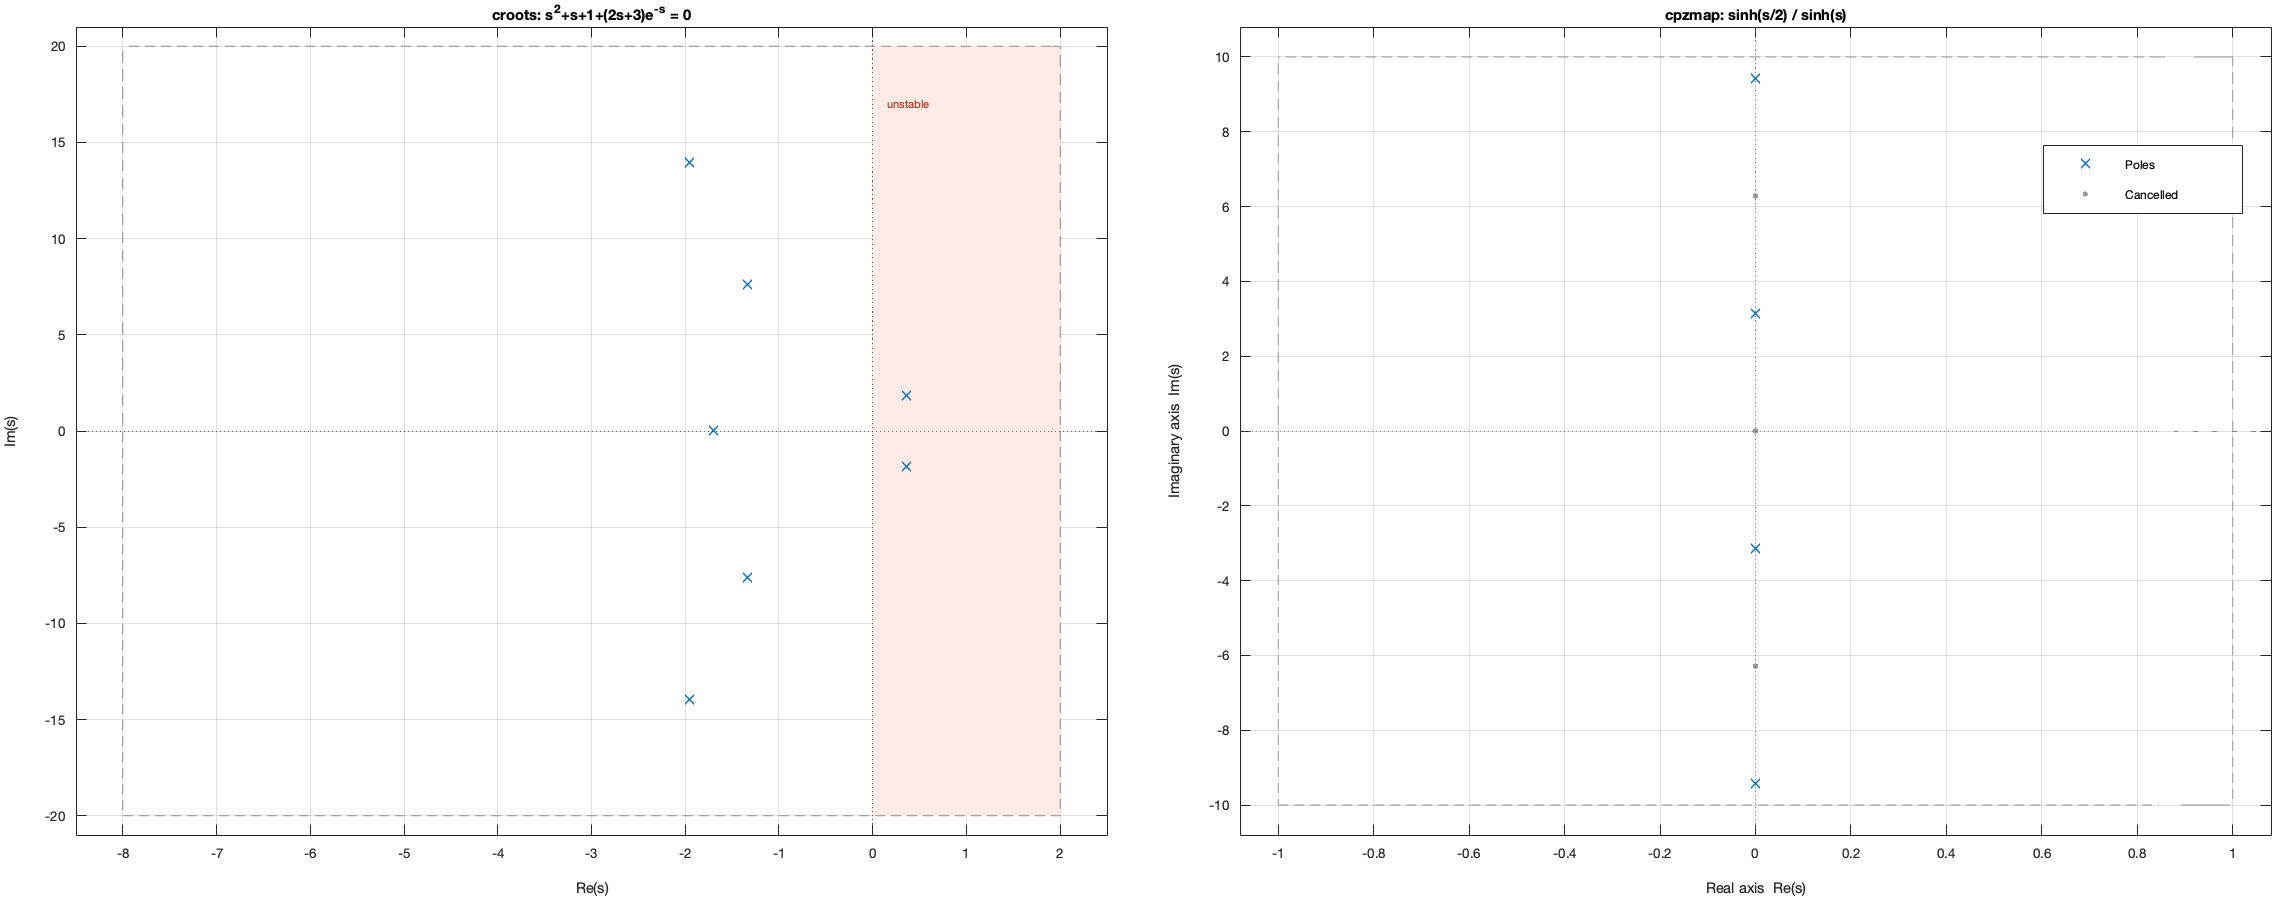
\includegraphics[width=\textwidth]{readme_overview.png}
\caption{Left: roots of $s^2+s+1+(2s+3)e^{-s}$ in the rectangle
$[-8,2]\times[-20,20]$ (dashed); the shaded area is the right half-plane.
Right: \code{cpzmap} of $\sinh(s/2)/\sinh(s)$; grey dots are cancelled
candidates.}
\label{fig:overview}
\end{figure}

\section{Time-delay stability}

For $D(s)+N(s)e^{-sT}=0$ with coefficient vectors \code{N} and \code{D}:
\begin{lstlisting}
crit = critical_delays(2, [1 1], 10);         % s + 1 + 2 e^{-sT} = 0
Z = unstable_root_count(2, [1 1], 1.5);       % 2 unstable roots
\end{lstlisting}
The first critical delay is $2\pi/(3\sqrt3)\approx1.2092$
(Chapter~\ref{ch:delay}).

\chapter{Mathematical background}\label{ch:background}

This chapter collects the facts from complex analysis on which the method
relies; see \citet{ahlfors1979} for proofs of the classical results.

\section{Analytic and meromorphic functions}

A function $F$ of the complex variable $s=x+\ii y$ is \emph{analytic}
(holomorphic) on an open set $U$ if it has a complex derivative at every
point of $U$. It is \emph{entire} if it is analytic on the whole plane.
Polynomials, $e^{s}$, $\sin s$, $\cos s$, $\sinh s$, $\cosh s$, and all sums,
products and compositions of entire functions are entire. A function is
\emph{meromorphic} on $U$ if it is analytic on $U$ except at isolated poles.

Two properties of analytic functions are essential:
\begin{enumerate}
  \item The zeros of an analytic function that is not identically zero are
        isolated, and each has a finite \emph{multiplicity} $m\ge1$:
        $F(s)=(s-s_0)^m g(s)$ with $g$ analytic and $g(s_0)\neq0$.
  \item A bounded region contains finitely many zeros.
\end{enumerate}
Neither holds for functions that are not analytic: $|s|^2-1$ vanishes on a
whole circle. Functions with branch points (such as $\sqrt s$ or $\log s$)
are analytic only on a domain that excludes a cut.

Some expressions that contain square roots are nevertheless entire. For
instance $\cosh\sqrt q=\sum_k q^k/(2k)!$ and $\sinh(\sqrt q)/\sqrt q=
\sum_k q^k/(2k+1)!$ contain only integer powers of $q$: the choice of the
branch of $\sqrt q$ does not change their value. Such \emph{even functions of
a root} appear in the transfer functions of Chapters~\ref{ch:distributed}
and~\ref{ch:beam}.

\section{The argument principle}

\begin{theorem}[Argument principle]\label{thm:arg}
Let $C$ be a simple closed piecewise-smooth curve, oriented
counterclockwise, and let $F$ be meromorphic on a neighborhood of $C$ and
its interior, with no zero or pole on $C$. Then
\begin{equation}
  \frac{1}{2\pi\ii}\oint_C\frac{F'(s)}{F(s)}\,ds \;=\; Z-P
  \;=\; \frac{1}{2\pi}\,\Delta_C\arg F(s),
  \label{eq:argprinciple}
\end{equation}
where $Z$ and $P$ are the numbers of zeros and poles inside $C$, counted
with multiplicity, and $\Delta_C\arg F$ is the total change of a continuous
branch of $\arg F(s)$ as $s$ travels once around $C$.
\end{theorem}

The right-hand form is the one used numerically: the change of argument
is the sum of the phase increments of $F$ between consecutive samples of
$C$, each taken in $(-\pi,\pi]$. It equals $2\pi$ times the \emph{winding
number} of the image curve $F(C)$ around the origin
(Figure~\ref{fig:argprinciple}).

\begin{figure}[H]
\centering
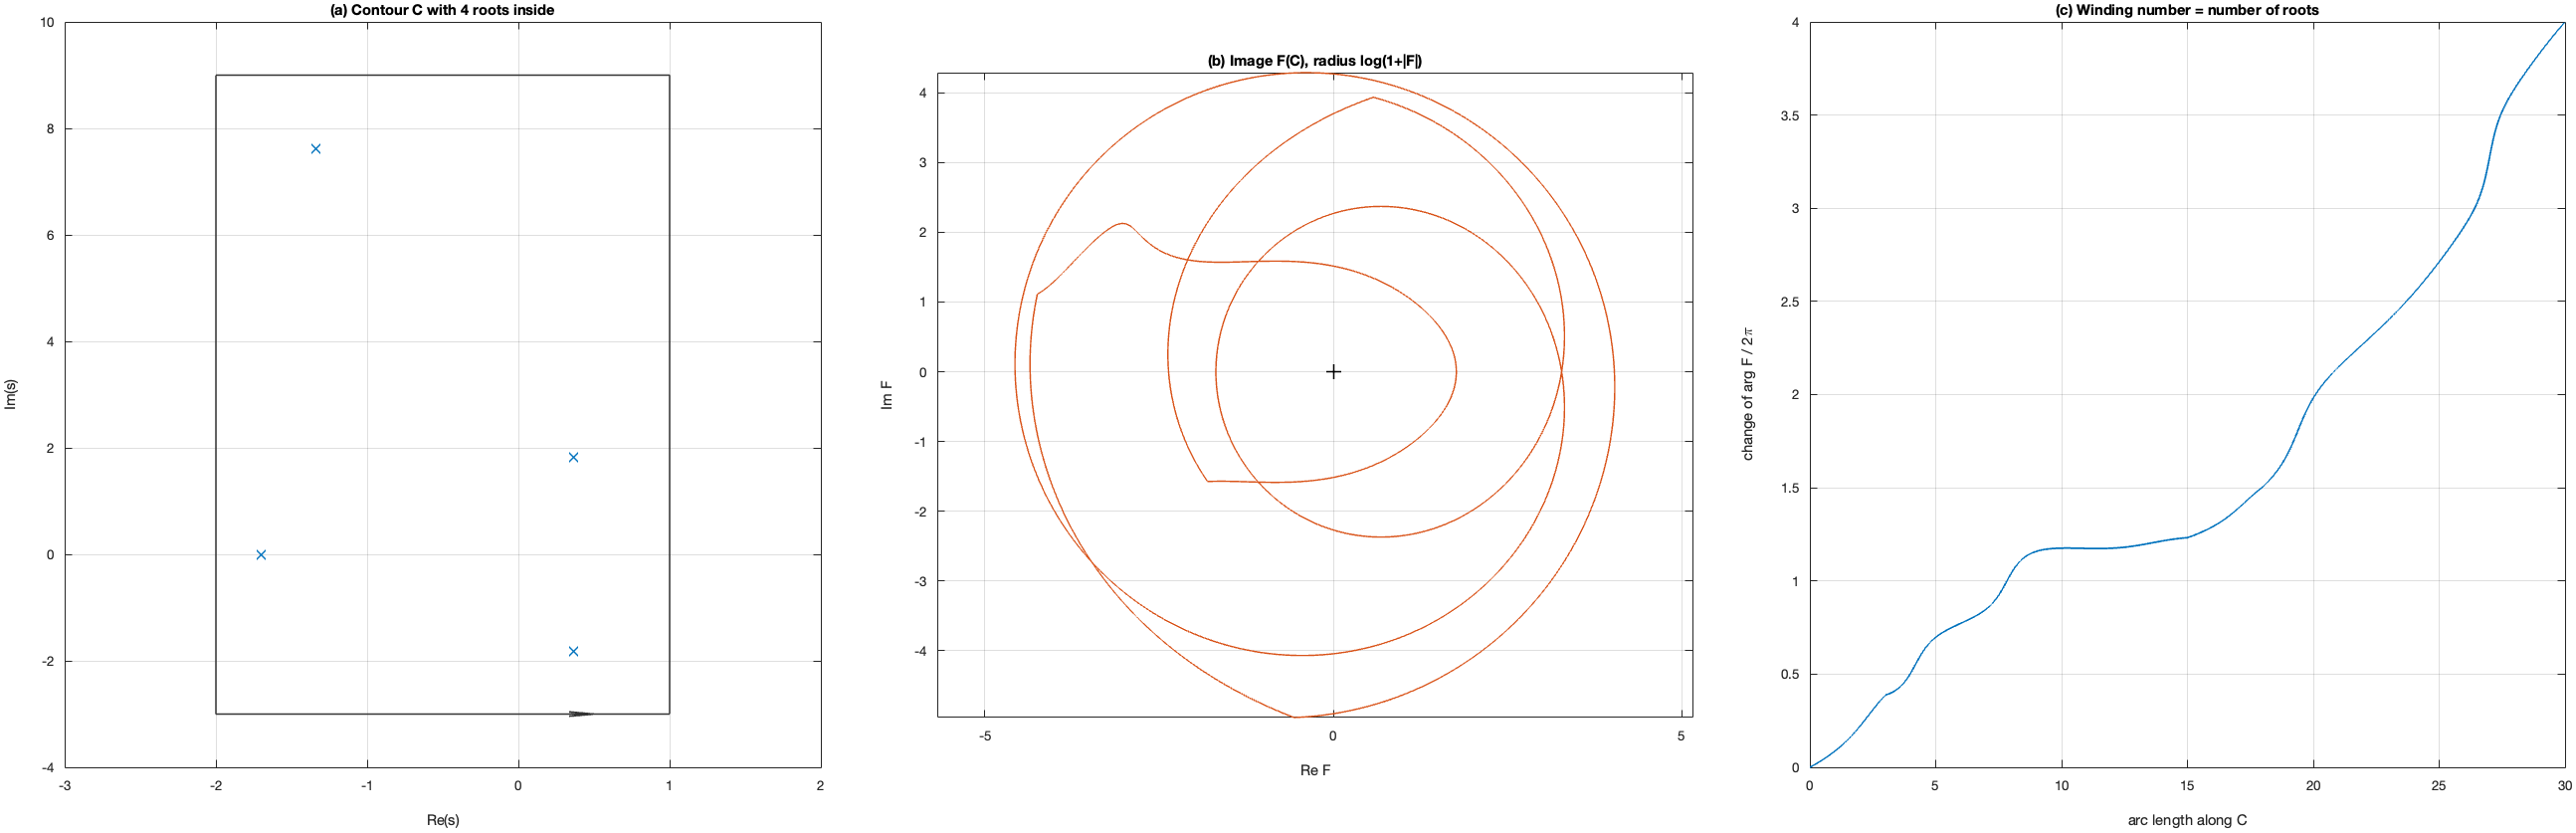
\includegraphics[width=\textwidth]{argument_principle.png}
\caption{The argument principle for $F(s)=s^2+s+1+(2s+3)e^{-s}$ on the
rectangle $[-2,1]\times[-3,9]$. (a) Four roots lie inside $C$. (b) The image
curve $F(C)$, drawn with radius $\log(1+|F|)$, winds four times around the
origin. (c) The unwrapped argument of $F$ along $C$ grows by $4\times2\pi$.}
\label{fig:argprinciple}
\end{figure}

Three consequences shape the design of ContourRoots.

\paragraph{Analytic functions.} If $F$ is analytic, $P=0$ and the integral
counts the zeros. This is the case for characteristic functions such as
$D(s)+N(s)e^{-sT}$.

\paragraph{Quotients.} For a transfer function $G=N/D$ with $N$ and $D$
analytic, the integral of $G'/G$ counts $Z_N-Z_D$ \emph{after}
cancellation. A count of zero does not mean that the region is empty. This
is why ContourRoots asks for $N$ and $D$ separately (\code{ndpair}) and
counts the zeros of each.

\paragraph{Multiplicity and the first moment.} If $F$ is analytic with zeros
$s_1,\dots,s_Z$ (repeated according to multiplicity) inside $C$,
\begin{equation}
  \frac{1}{2\pi\ii}\oint_C s\,\frac{F'(s)}{F(s)}\,ds=\sum_{j=1}^{Z}s_j .
  \label{eq:moment}
\end{equation}
Divided by $Z$ it gives the centroid of the zeros; when $Z=1$ it gives the
zero itself. Higher moments lead to the classical methods of
\citet{delves1967} and \citet{kravanja2000}, which compute all zeros inside
$C$ from a small eigenvalue problem. ContourRoots uses only the first
moment, as a starting point for Newton's method.

\section{Cancellation of poles and zeros}

Let $N$ and $D$ be analytic near $s_0$, with zeros of orders $m_N\ge0$ and
$m_D\ge0$ at $s_0$. Then $G=N/D$ has at $s_0$
\begin{itemize}
  \item a pole of order $m_D-m_N$ if $m_D>m_N$;
  \item a zero of order $m_N-m_D$ if $m_N>m_D$;
  \item neither (a removable point, after cancellation) if $m_N=m_D$.
\end{itemize}
Counting the zeros of $N$ and of $D$ separately in a small disk around each
candidate determines $m_N$ and $m_D$, and therefore the type and order of
the point. This is the cancellation test of Section~\ref{sec:cancel}.

\section{Modes and transfer poles}

For a linear system, the roots of the characteristic function are the
\emph{modes}; they decide internal stability. A transfer function from one
input to one output may not contain every mode: a mode that the input
cannot excite, or that the output cannot observe, appears as a common zero
of $N$ and $D$ and cancels. Both computations are available: \code{croots}
on the characteristic function returns the modes, and \code{cpoles} on
$N/D$ returns the transfer poles. Examples of hidden modes appear in
Sections~\ref{sec:heat} and~\ref{sec:beamvalidation}.

\chapter{Algorithm and numerical safeguards}\label{ch:algorithm}

The solver, \code{complex\_spectrum}, isolates the zeros of an analytic
function $f$ in a rectangle $\Omega=[x_0,x_1]\times[y_0,y_1]$. In zero mode
$f=N$ (or the given function); in pole mode $f=D$. This chapter describes
each component and the conditions under which a result is declared
complete.

\section{Contour counts}\label{sec:count}

The boundary of a rectangle $B$ is sampled at $n$ equally spaced points per
edge, $4n$ points in total, traversed counterclockwise. With
$v_j=f(z_j)$, the phase and log-modulus increments are
\[
  \delta_j=\operatorname{Arg}\frac{v_{j+1}}{v_j}\in(-\pi,\pi],\qquad
  \mu_j=\log|v_{j+1}|-\log|v_j| ,
\]
and the discrete winding number is $w=\frac{1}{2\pi}\sum_j\delta_j$. The
number of samples starts at $n=n_0$ (\code{ContourPoints}, default 32) and
is doubled up to \code{ContourRefinements} times (default 7, i.e.\ up to
4096 points per edge). A count is \emph{accepted} when
\begin{enumerate}
  \item the rounded winding number $\operatorname{round}(w)$ is the same at
        three consecutive sampling levels,
  \item at the last two levels $|w-\operatorname{round}(w)|<10^{-7}$, and
  \item at the last two levels every increment satisfies $|\delta_j|<\pi/3$
        and $|\mu_j|<2$.
\end{enumerate}
Condition 3 is the practical form of the requirement that the argument of
$f$ vary slowly between samples; without it, a fast phase rotation could be
aliased and a whole turn lost. If any sample is zero, infinite or
\code{NaN} (a zero on the boundary, or overflow), or if the conditions are
not met at the finest level, the count fails and the rectangle is
\emph{unresolved}.

The same samples give the first-moment estimate~\eqref{eq:moment}, computed
as $\sum_j \tfrac{z_j+z_{j+1}}{2}(\mu_j+\ii\delta_j)/(2\pi\ii\,Z)$, used as a
Newton starting point.

\section{Newton's method}\label{sec:newton}

From a starting point $z$ inside a cell $B$ with count $m$, the solver
applies the modified Newton iteration
\[
  z\leftarrow z-\alpha\, m\,\frac{f(z)}{f'(z)} ,
\]
which converges quadratically to a zero of multiplicity $m$. Safeguards:
\begin{itemize}
  \item the step is limited to half the larger side of $B$;
  \item the damping factor $\alpha$ is halved (at most 12 times) until
        $|f|$ does not increase; if it cannot be decreased, the start is
        abandoned;
  \item the iteration stops if it leaves $B$, and converges when the step is
        below \code{RootTolerance}$\cdot(1+|z|)$.
\end{itemize}
The derivative is the user-supplied \code{Derivative}, the exact derivative
for symbolic input and coefficient vectors, or otherwise the four-point
complex difference
\[
  f'(z)\approx\frac{f(z+h)-f(z-h)-\ii\,[f(z+\ii h)-f(z-\ii h)]}{4h},
  \qquad h=10^{-4}\max(1,|z|),
\]
whose error is $O(h^4)$ for analytic $f$ (the $h^2$ terms of the real and
imaginary central differences cancel).

\section{Local confirmation}\label{sec:confirm}

A Newton limit $z^\ast$ is accepted only if a contour count on the small
square of half-width $\rho=\code{RootTolerance}\cdot(1+|z^\ast|)$ centered
at $z^\ast$ equals the count $m$ of the cell. This confirms both that
$z^\ast$ is a zero and that no other zero of the cell was missed; $m$ becomes
the multiplicity of $z^\ast$, and $\sqrt2\rho$ is reported as
\code{locationRadius}. Consequently, zeros closer than about $\rho$ are
reported as one location whose multiplicity is the size of the cluster.

\section{Recursive subdivision}\label{sec:subdivision}

\begin{algobox}{Algorithm 1 — recursive isolation of the zeros of $f$ in a cell $B$ with count $m$}
\begin{enumerate}[leftmargin=1.7em]
  \item If $m=0$, return.
  \item For each start in (first-moment center of $B$, geometric center of
        $B$, user seeds inside $B$): run Newton (Section~\ref{sec:newton});
        if the limit is confirmed with count $m$ (Section~\ref{sec:confirm}),
        record it and return.
  \item If the depth exceeds \code{MaxDepth} or the number of visited cells
        exceeds \code{MaxCells}, mark $B$ unresolved and return.
  \item Split $B$ across its longer side at the fraction $0.5$ of the side.
        Count the two halves. If both counts are accepted and add up to $m$,
        recurse into both halves and return.
  \item Otherwise retry with the split fractions $0.438\ldots$ and
        $0.573\ldots$, then with the other side. If no split conserves the
        count, mark $B$ unresolved.
\end{enumerate}
\end{algobox}

The \emph{conservation check} of step 4 detects zeros lying on the split
line (the counts of the halves then fail or do not add up) and moves the
line. The irrational-looking fractions make it unlikely that a second
attempt hits a zero again. Unresolved cells are never discarded: they are
returned in \code{info.unresolvedBoxes}.

\section{Cancellation}\label{sec:cancel}

In pole mode with a pair $N/D$, the zeros of $D$ are isolated with
Algorithm~1. For each location $z^\ast$ with multiplicity $m_D$, the zeros of
$N$ are counted on the same small square, giving $m_N$. The reported
multiplicity is $\max(m_D-m_N,0)$; if it is zero, $z^\ast$ is moved to
\code{cancelledLocations}, and the removed order $\min(m_D,m_N)$ is recorded.
Zero mode is symmetric. If the count of the other factor fails, the location
is kept and flagged in \code{cancellationUncertain}, and the result is not
complete. The test has the resolution of the small square: a pole and a zero
closer than $\rho$ are indistinguishable from an exact cancellation.

\section{Exploratory mode}\label{sec:exploratory}

When the function is not known to be analytic (an opaque handle without
\code{AssumeAnalytic}, or a single quotient handle), contour counts may
measure $Z-P$ instead of $Z$ and cannot be trusted. The solver then starts
Newton from a \code{GridSize} grid of points and from the seeds, and keeps
the limits confirmed by a positive local count. The result has status
\code{exploratory} and is never declared complete.

\section{The completeness contract}\label{sec:contract}

A search is \code{numerically\_complete} when (i) the count on
$\partial\Omega$ was accepted, (ii) every cell was resolved, (iii) the
multiplicities of the located zeros add up to that count, and (iv) every
cancellation test was resolved. Under the analyticity assumption, and if
the accepted counts are correct, all zeros in $\Omega$ are then reported,
each within its \code{locationRadius} as a cluster of the stated
multiplicity.

\begin{keybox}{What this is not}
It is not a proof. The counts are computed from finitely many floating-point
samples; a function that oscillates between samples faster than the
safeguards of Section~\ref{sec:count} can detect could in principle fool
them. Analyticity of a handle is the user's declaration. Residuals depend on
the scaling of the searched factor and are not bounds on the location
error. \code{info.certified} is always false. Rigorous enclosures would
require interval arithmetic, which is outside the scope of this version.
\end{keybox}

\section{Cost}

The cost is dominated by function evaluations on contours: $4n$ per count,
with $n$ doubling until acceptance, for the outer rectangle, for every
cell of the subdivision and for every local confirmation. Vectorized
handles are evaluated on all samples of a contour at once. Tall rectangles
over oscillatory functions (e.g.\ $e^{-sT}$ with large $T|\Imag s|$) need
more samples per edge; smaller rectangles or larger
\code{ContourRefinements} help. Seeds from a previous parameter value
reduce the number of subdivisions in parameter sweeps.

\section{Related methods and software}\label{sec:related}

Contour-integral root finders go back to \citet{delves1967}; see
\citet{kravanja2000} for a thorough treatment including moment-based
eigenvalue formulations. \code{cxroots} \citep{cxroots} implements such a
method in Python with subdivision. GRPF \citep{grpf} analyzes the phase of a
single meromorphic function on an adaptive triangulation and locates both
zeros and poles. For quasi-polynomials and time-delay systems, QPmR
\citep{vyhlidal2009} maps the zero-level curves of the real and imaginary
parts, and spectral discretization methods \citep{breda2005,breda2015,michiels2014}
approximate the rightmost roots of matrix delay equations. ContourRoots
combines well-known ingredients; its emphasis is on a MATLAB-style
interface, explicit cancellation for $N/D$ pairs, and diagnostics that make
incomplete searches visible.

\chapter{Model input and the analyticity contract}\label{ch:inputs}

The algorithm of Chapter~\ref{ch:algorithm} is only as good as its
assumption that the searched factor is analytic on a neighborhood of the
closed rectangle. This chapter lists the accepted input forms and states,
for each, how that assumption is established.

\section{Input forms}

\begin{center}\small
\begin{tabularx}{\textwidth}{>{\raggedright}p{3.1cm}X}
\toprule
Input & Treatment\\\midrule
Coefficient vector & Polynomial in descending powers, exact derivative; analytic by construction. \code{croots(c,region)} behaves like \code{roots(c)} restricted to the rectangle.\\
Function handle & Evaluated as given. Analytic only if the user passes \code{AssumeAnalytic}; otherwise exploratory. Vectorized handles are evaluated on whole contours; scalar-only handles are evaluated point by point.\\
\code{ndpair(N,D)} & Each factor is a handle, a coefficient vector or a symbolic expression. Polynomial and checked symbolic factors are analytic automatically; handles need \code{AssumeAnalytic}, which then applies to \emph{both} factors.\\
Symbolic (\code{sym}, \code{symfun}) & Split with \code{numden}; each factor is checked by a conservative grammar (below) and differentiated exactly.\\
\code{tf}, \code{zpk}, \code{ss} & Continuous-time SISO only. Rational models and \code{tf} models with input, output or transport delays become an analytic pair (delay in the numerator). Models with internal delays are evaluated with \code{evalfr} in exploratory mode.\\
\bottomrule
\end{tabularx}\end{center}

\section{The symbolic analyticity check}

A symbolic factor is accepted as entire if it is a number, the variable, or
is built from entire factors by sums, products, $\exp$, $\sin$, $\cos$,
$\sinh$, $\cosh$ and powers with constant nonnegative integer exponents.
The check is \emph{sufficient, not necessary}: $\cosh\sqrt s$ is entire but
is rejected, with the error \code{complex\_spectrum:AnalyticContract}. The
remedy is to provide the factor as a handle that evaluates the entire
function directly (with a series near removable points,
Chapter~\ref{ch:distributed}) and to declare \code{AssumeAnalytic}. All
parameters other than the complex variable must be substituted numerically
before the call.

\section{What a declaration of analyticity means}

\code{'AssumeAnalytic',true} asserts that the searched factor(s) are
analytic on an open set containing the closed rectangle. It is a statement
about mathematics, not about the code, and must be checked by the user:
\begin{itemize}
  \item removable singularities (e.g.\ $\sinh(s)/s$ at $0$) must be removed
        in the implementation, otherwise the evaluation returns \code{NaN};
  \item roots such as $\sqrt s$ or $s^{1/4}$ are acceptable only inside
        combinations invariant under the change of branch;
  \item for a \emph{single} handle in pole mode, the declaration concerns
        $1/G$: it asserts that $G$ has no zeros in the rectangle. For
        transfer functions with zeros, use \code{ndpair}.
\end{itemize}
A false declaration makes the counts meaningless and can produce wrong
results without any warning.

\section{Singular points}

Some models have points where the function is not meromorphic: branch
points of genuinely multivalued functions, or accumulation points of poles
(Section~\ref{sec:kelvinvoigt}). No finite contour computation can resolve
a neighborhood of such a point. The option \code{Singularities} declares
them; a rectangle that contains one is rejected with the error
\code{complex\_spectrum:SingularityInRegion}. The solver does not discover
such points in opaque handles.

\section{Scaling}

The argument principle is invariant under multiplication of $f$ by a
nonzero constant, and the regression tests check that roots do not change
when $f$ is scaled by $10^{\pm100}$. Overflow is a different matter: a
term such as $e^{-sT}$ grows like $e^{T|\Real s|}$ in the left half-plane,
and samples that overflow make a count fail. Rectangles extending far to
the left may need to be split, or the function rescaled by an analytic
nonvanishing factor.

\chapter{Interface reference}\label{ch:api}

The complete reference, with examples for every function, is in
\code{docs/api/} and in the MATLAB help (\code{help croots}). This chapter
summarizes it.

\section{Functions}

\begin{center}\small
\begin{tabularx}{\textwidth}{>{\ttfamily}p{6.0cm}X}
\toprule
\normalfont Syntax & Purpose\\\midrule
{}[r,info] = croots(F,region,...) & roots of $F$ in the rectangle\\
{}[p,info] = cpoles(G,region,...) & poles of $G$ after cancellation\\
{}[z,info] = czeros(G,region,...) & zeros of $G$ after cancellation\\
cpzmap(G,region,...) & pole-zero map; \code{[p,z,infoP,infoZ]} without plot\\
G = ndpair(N,D) & transfer function from two analytic factors\\
{}[x,info] = complex\_spectrum(...) & core solver, \code{'Mode'} \code{'zeros'}/\code{'poles'}\\
crit = critical\_delays(N,D,Tmax) & crossings of $D+Ne^{-sT}$, $0\le T\le T_{\max}$\\
Z = unstable\_root\_count(N,D,T) & roots with $\Real s\ge0$ (bound-based count)\\
R = rhp\_root\_bound(N,D) & radius containing all such roots, all $T$\\
delay\_roots, delay\_root\_count & grid/Newton solver and count for one delay\\
pade\_delay, pade\_characteristic & diagonal Padé coefficients and polynomial\\
pade\_critical\_delays & critical delays predicted by Padé models\\
{}[g,t,info] = cimpulse(G,t,...) & ordinary impulse response; Dirac terms in \code{info}\\
{}[y,t,info] = cstep(G,t,...) & unit-step response\\
{}[y,t,info] = clsim(G,u,t,...) & response to a sampled input (ZOH/FOH)\\
{}[f,t,info] = cinvlaplace(F,t,...) & inverse Laplace transform of $F(s)$\\
setup\_contourroots, contourroots & path setup; overview and version\\
\bottomrule
\end{tabularx}\end{center}

The region is always \code{[xmin xmax ymin ymax]}. When \code{info} is not
requested and a search of \code{croots}, \code{cpoles}, \code{czeros} or
\code{cpzmap} is not complete, a warning (\code{ContourRoots:Exploratory} or
\code{ContourRoots:Incomplete}) is issued; \code{'Warn',false} silences it.

\section{Options}

\begin{center}\small
\begin{tabularx}{\textwidth}{>{\ttfamily}p{3.6cm}p{1.6cm}X}
\toprule
\normalfont Option & Default & Meaning\\\midrule
AssumeAnalytic & false & declare the searched factor(s) analytic\\
SeedPoints & [] & extra Newton starts\\
Derivative & [] & $F'$ for a single handle\\
Singularities & [] & points that must not lie in the region\\
RootTolerance & 1e-7 & relative half-width of confirmation boxes\\
ContourPoints & 32 & initial samples per edge\\
ContourRefinements & 7 & maximum doublings of the sampling\\
MaxDepth & 24 & maximum subdivision depth\\
MaxCells & 5000 & maximum number of cells\\
MaxIterations & 80 & Newton iterations per start\\
GridSize & [25 41] & start grid in exploratory mode\\
Plot, Display & false & figure or table of results\\
Warn & true & incompleteness warning (wrappers only)\\
\bottomrule
\end{tabularx}\end{center}

\section{Diagnostics}

\begin{center}\small
\begin{tabularx}{\textwidth}{>{\ttfamily\raggedright}p{5.6cm}X}
\toprule
\normalfont Field & Meaning\\\midrule
status & \code{numerically\_complete}, \code{unresolved} or \code{exploratory}\\
complete & conditions (i)--(iv) of Section~\ref{sec:contract} hold\\
certified & always false\\
count & total multiplicity returned, after cancellation\\
targetCountBeforeCancellations & outer count of the searched factor\\
multiplicity & multiplicity (cluster size) of each location\\
locationRadius & resolution of each location (not an error bound)\\
residuals & $|f|$ of the searched factor at each location\\
cancelledLocations, cancellationOrders & removed candidates and orders\\
cancellationUncertain & cancellation test unresolved at a location\\
unresolvedBoxes & cells that could not be resolved\\
contourResolved, cellsVisited & outer count accepted; cells used\\
exploratory, region, mode, analyticSource & context of the search\\
\bottomrule
\end{tabularx}\end{center}

\chapter{Time-delay systems and the limits of Padé approximations}\label{ch:delay}

This chapter studies the scalar characteristic equation
\begin{equation}
  F(s,T)=D(s)+N(s)\,e^{-sT}=0,\qquad T\ge0,
  \label{eq:qp}
\end{equation}
with real polynomials $D$ of degree $m$ and $N$ of degree $p$. It shows
that the stability of such systems can be decided for every delay without
approximating the delay, and then examines precisely what a Padé
approximation of $e^{-sT}$ preserves and what it loses.

\section{Formulation}

The simplest example is the delay-differential equation
\begin{equation}
  \dot x(t)=-a\,x(t)-b\,x(t-T).
  \label{eq:dde}
\end{equation}
Its solution from $t=0$ is determined only by a whole \emph{history}
$x(\theta)=\varphi(\theta)$, $\theta\in[-T,0]$: on $[0,T]$ the delayed term is
known and \eqref{eq:dde} is an ordinary differential equation; its solution
determines the delayed term on $[T,2T]$, and so on (the \emph{method of
steps} \citep{bellman1963}). The state is a function, and the system is
infinite-dimensional. Exponential solutions $e^{st}$ exist when
$s+a+be^{-sT}=0$. More generally, the loop of Figure~\ref{fig:loop}, a
rational plant $N/D$ with delayed unit feedback, has the characteristic
equation~\eqref{eq:qp}.

\begin{figure}[H]
\centering
\begin{tikzpicture}[
  blk/.style={draw=ink,thick,minimum width=22mm,minimum height=10mm,align=center,fill=soft},
  sum/.style={draw=ink,thick,circle,minimum size=6mm,inner sep=0},
  arr/.style={-{Stealth[length=2.2mm]},thick}]
  \node (in) at (0,0) {$r$};
  \node[sum,right=12mm of in] (s) {};
  \node[blk,right=14mm of s] (G) {$\dfrac{N(s)}{D(s)}$};
  \coordinate[right=16mm of G] (out);
  \node[right=4mm of out] (y) {$y$};
  \node[blk,below=10mm of G,fill=softred,draw=rust] (d) {$e^{-sT}$};
  \draw[arr] (in) -- (s);
  \draw[arr] (s) -- node[above]{$e$} (G);
  \draw[arr] (G) -- (out) -- (y);
  \draw[arr] (out) |- (d);
  \draw[arr] (d) -| node[pos=0.95,right]{$-$} (s);
\end{tikzpicture}
\caption{Loop with a delay in the feedback path. The loop transfer function
is $L(s)=\frac{N(s)}{D(s)}e^{-sT}$; $1+L=0$ is equivalent to~\eqref{eq:qp}.
The delay has unit gain at every frequency and unbounded phase $-\omega T$.}
\label{fig:loop}
\end{figure}

\begin{definition}
The system is \emph{retarded} if $p<m$ and \emph{neutral} if $p=m$.
\end{definition}
Throughout this chapter $p<m$. Three cases illustrate the typical
behaviors (Table~\ref{tab:cases}).

\begin{table}[H]\centering\small
\caption{Case studies; all are stable at $T=0$.}\label{tab:cases}
\begin{tabular}{llll}\toprule
Case & Equation & Model & Behavior as $T$ grows\\\midrule
P1 & $s+1+2e^{-sT}=0$ & $\dot x=-x(t)-2x(t-T)$ & loses stability at $T\approx1.209$\\
P2 & $s+2+e^{-sT}=0$ & $\dot x=-2x(t)-x(t-T)$ & stable for every $T\ge0$\\
P3 & $s^2+0.8s+4+3e^{-sT}=0$ & $\ddot x+0.8\dot x+4x=-3x(t-T)$ & stability switches\\
\bottomrule\end{tabular}
\end{table}

\section{Structure of the spectrum}

$F(\cdot,T)$ is entire and, for $T>0$, has infinitely many roots. For
retarded systems they form chains that move to the left: balancing
$|D(s)|\sim|s|^m$ with $|N(s)e^{-sT}|\sim|s|^pe^{-T\Real s}$ gives
\[
  \Real s\approx-\frac{m-p}{T}\ln|s|,\qquad |s|\to\infty .
\]
Hence every half-plane $\Real s>c$ contains finitely many roots, the
\emph{spectral abscissa} $\alpha(T)=\max\{\Real s:F(s,T)=0\}$ is well
defined, and the zero solution of a linear retarded system is exponentially
stable if and only if $\alpha(T)<0$ \citep{hale1993,michiels2014}.
Figure~\ref{fig:polemaps} shows the spectra of the three cases together
with the poles of Padé models (Section~\ref{sec:pade}).

\begin{figure}[H]
\centering
\includegraphics[width=\textwidth]{pole_maps.pdf}
\caption{Roots of~\eqref{eq:qp} ($\times$) and poles of diagonal Padé
models ($\circ$) at $T=1$ (P1, P2) and $T=0.8$ (P3). The exact chains
continue to the left; the rational spectra are finite.}
\label{fig:polemaps}
\end{figure}

\begin{proposition}[A region containing all unstable roots]\label{prop:bound}
Let $p<m$, $D$ monic, $D(s)=s^m+\sum_{k<m}d_ks^k$, $N(s)=\sum_{k\le p}n_ks^k$,
and let $R>0$ be the positive root of
\[
  r^m-\sum_{k<m}|d_k|r^k-\sum_{k\le p}|n_k|r^k=0 .
\]
Then for every $T\ge0$, every root of~\eqref{eq:qp} with $\Real s\ge0$
satisfies $|s|\le R$.
\end{proposition}
The proof is in Appendix~\ref{ap:proofs}. For P1, $|s+1|\le2$ gives $R=3$;
for P3, $R\approx3.076$. The function \code{rhp\_root\_bound} computes $R$,
and \code{unstable\_root\_count} applies the argument principle to the
rectangle $[0,R+1]\times[-(R+1),R+1]$: the number $Z(T)$ of unstable roots
is obtained without guessing a search window and without approximation
(the count itself is a floating-point computation, reliable away from
critical delays).

\section{Roots for a given delay}

The study of this chapter locates roots with the delay-specific solver
\code{delay\_roots} (damped Newton from a grid, audited by an
argument-principle count); \code{croots} gives the same roots with the
subdivision algorithm of Chapter~\ref{ch:algorithm}. Table~\ref{tab:solver}
shows that the number of roots found agrees with the independent count and
that the residuals are near machine precision.

\input{../output/time_delay/data/table_solver.tex}

\section{Critical delays}

As $T$ varies the roots move continuously, and new roots appear only from
$\Real s=-\infty$. Stability can therefore change only when a root crosses
the imaginary axis. At a crossing $s=\ii\omega$, $\omega>0$,
\begin{equation}
  e^{-\ii\omega T}=-\frac{D(\ii\omega)}{N(\ii\omega)} .
  \label{eq:crossing}
\end{equation}
This complex equation splits into two real equations with very different
roles.

\paragraph{Modulus: where.} The left side has unit modulus for every $T$,
so the crossing frequencies do not depend on the delay and solve
\begin{equation}
  G(\omega)=|D(\ii\omega)|^2-|N(\ii\omega)|^2=0 ,
  \label{eq:G}
\end{equation}
an even polynomial in $\omega$, i.e.\ a polynomial of degree $m$ in
$x=\omega^2$. Its positive roots give a \emph{finite} set of frequencies.

\paragraph{Phase: when.} For each frequency $\omega_i$, with
$\theta_i=\operatorname{mod}(-\arg[-D(\ii\omega_i)/N(\ii\omega_i)],2\pi)$, the
phase condition gives \emph{infinitely many} critical delays
\begin{equation}
  T_{i,k}=\frac{\theta_i+2\pi k}{\omega_i},\qquad k=0,1,2,\ldots
  \label{eq:Tk}
\end{equation}
This elimination is the scalar form of the direct method
\citep{walton1987,olgac2002,michiels2014}. \code{critical\_delays} computes
all $T_{i,k}$ in an interval and refines each pair $(\omega,T)$ by a
two-variable Newton correction.

\begin{example}[P1]
$G(\omega)=1+\omega^2-4$ gives $\omega_c=\sqrt3$. Since
$-D(\ii\sqrt3)/N=e^{-2\pi\ii/3}$, $\theta=2\pi/3$ and
$T_k=(2\pi/3+2\pi k)/\sqrt3$: $T_0=2\pi/(3\sqrt3)\approx1.2092$,
$T_1\approx4.8368$, $T_2\approx8.4644$.
\end{example}
\begin{example}[P3]
$G(\omega)=\omega^4-7.36\,\omega^2+7$ has the roots $\omega_1\approx2.4976$ and
$\omega_2\approx1.0593$; each generates its own sequence of critical delays,
and the two sequences interleave.
\end{example}
For P2, $G(\omega)=\omega^2+3>0$: there is no crossing, and since P2 is
stable at $T=0$ it is stable for every delay.

\section{Direction of the crossings}

Differentiating $F(s(T),T)=0$ gives
\begin{equation}
  \frac{ds}{dT}=-\frac{F_T}{F_s}
  =\frac{s\,e^{-sT}N(s)}{D'(s)+e^{-sT}[N'(s)-TN(s)]} .
  \label{eq:speed}
\end{equation}
The crossing is destabilizing if $\Real(ds/dT)>0$ at $s=\ii\omega$. The
following classical result \citep{cooke1986} makes the direction a property
of the frequency alone.

\begin{proposition}[Direction depends only on the frequency]\label{prop:direction}
At a simple crossing $s=\ii\omega$, $\omega>0$,
$\operatorname{sign}\Real\dfrac{ds}{dT}=\operatorname{sign}G'(\omega)$.
\end{proposition}

All branches $k$ of a frequency therefore cross in the same direction. In
P1, $G'(\sqrt3)>0$: every $T_k$ adds an unstable pair. In P3, crossings at
$\omega_1$ always destabilize and crossings at $\omega_2$ always stabilize
(Table~\ref{tab:critical}, Figure~\ref{fig:critical}).

\input{../output/time_delay/data/table_critical.tex}

\begin{figure}[H]
\centering
\includegraphics[width=0.95\textwidth]{critical_delays.pdf}
\caption{Frequencies and directions of the exact crossings (up: into the
right half-plane; down: back to the left half-plane).}
\label{fig:critical}
\end{figure}

\section{Stability map}

Each simple crossing moves one conjugate pair, so the number of roots in
the right half-plane is the step function
\begin{equation}
  Z(T)=Z(0)+2\sum_{T_{i,k}<T}\operatorname{sign}G'(\omega_i),
  \label{eq:Z}
\end{equation}
where $Z(0)$ is the number of unstable roots of $D+N$ (the roots created
when $T$ becomes positive come from $\Real s=-\infty$). For P3 on
$[0,10]$:
\[
  Z(T)=\begin{cases}
   0, & 0\le T<0.2918,\\
   2, & 0.2918<T<2.6953,\\
   0, & 2.6953<T<2.8076\quad\text{(stability window)},\\
   2,4,6,4, & \text{after }2.8076,\ 5.3233,\ 7.8390,\ 8.6265.
  \end{cases}
\]
The window has width $0.112$ and could easily be missed by a sweep in $T$.
Formula~\eqref{eq:Z} was checked independently with
\code{unstable\_root\_count} at 80 delays, with full agreement (black curve
and circles in Figure~\ref{fig:Zp3}). Figure~\ref{fig:alpha} shows the
spectral abscissa computed by a sweep, refined near the window.

\begin{figure}[H]
\centering
\includegraphics[width=\textwidth]{spectral_abscissa.pdf}
\caption{Spectral abscissa versus delay, exact and with Padé models of
orders 1, 4 and 8; diamonds are the exact critical delays of~\eqref{eq:Tk}.
In P3 the exact curve touches zero at $T\approx2.695$ and crosses again at
$T\approx2.808$; the \pade{1} model misses the window and the \pade{4}
model widens it.}
\label{fig:alpha}
\end{figure}

\section{The Padé approximation}\label{sec:pade}

The diagonal Padé approximation of $e^{-z}$ of order $n$ is the rational
function $P_n(z)/Q_n(z)$ whose Taylor series agrees with that of $e^{-z}$
up to $z^{2n}$ \citep{baker1996}:
\begin{equation}
  e^{-z}-\frac{P_n(z)}{Q_n(z)}=O(z^{2n+1}),\quad
  Q_n(z)=\sum_{k=0}^n\frac{(2n-k)!\,n!}{(2n)!\,k!\,(n-k)!}z^k,\quad
  P_n(z)=Q_n(-z).
  \label{eq:pade}
\end{equation}
With $z=sT$ the characteristic equation becomes the polynomial
$D(s)Q_n(sT)+N(s)P_n(sT)$ of degree $m+n$. Three structural properties
determine its behavior.

\paragraph{(i) Exact gain.} Since $P_n(\ii y)=\overline{Q_n(\ii y)}$,
\begin{equation}
  \left|\frac{P_n(\ii y)}{Q_n(\ii y)}\right|=1\ \ (y\in\mathbb R),\qquad
  \left|\frac{P_n(z)}{Q_n(z)}\right|\le1\ \ (\Real z\ge0),
  \label{eq:allpass}
\end{equation}
the second by the maximum principle, as all roots of $Q_n$ lie in the left
half-plane. The error of the approximation is entirely in the phase.

\paragraph{(ii) Bounded phase.} Writing $P_n(\ii y)/Q_n(\ii y)=e^{\ii\phi_n(y)}$,
$\phi_n=-2\arg Q_n(\ii y)$ decreases monotonically and
\begin{equation}
  \phi_n(y)=-y+O(y^{2n+1})\ (y\to0),\qquad \phi_n(y)\searrow-n\pi\ (y\to\infty),
  \label{eq:phase}
\end{equation}
whereas the exact phase $-y$ is unbounded (Figure~\ref{fig:phaseuniv}).
This behavior depends only on $y=\omega T$.

\paragraph{(iii) Right-half-plane zeros.} The $n$ zeros of $P_n(sT)$ have
positive real part. The step response of the approximation jumps to
$(-1)^n$ at $t=0^+$ and oscillates before $t=T$, while the true delay stays
at zero (Figure~\ref{fig:step}).

\begin{figure}[H]
\centering
\includegraphics[width=\textwidth]{pade_phase_universal.pdf}
\caption{(a) Unwrapped phase of $e^{-\ii y}$ and of $\pade{n}$
approximations; dotted lines mark $-n\pi$. (b) Phase error; the dashed line
marks $10^{-2}$ rad.}
\label{fig:phaseuniv}
\end{figure}

\begin{figure}[H]
\centering
\includegraphics[width=0.85\textwidth]{pade_step_response.pdf}
\caption{Step response of $e^{-s}$ and of its Padé approximations.}
\label{fig:step}
\end{figure}

Table~\ref{tab:validity} quantifies property (ii): the largest $y$ for
which the phase error is below a tolerance. For $0.01$ rad and $n\ge4$,
$y_{0.01}\approx1.6n-2$.

\begin{table}[H]\centering\small
\caption{Largest $y=\omega T$ with Padé phase error below $0.1$, $0.01$ and
$10^{-6}$ rad, and asymptotic phase.}\label{tab:validity}
\input{../output/time_delay/data/pade_validity_table.tex}
\end{table}

\section{What Padé preserves}

\begin{proposition}[Frequencies and directions are inherited]\label{prop:padedir}
For the rational equation $D+NP_n/Q_n=0$:
\begin{enumerate}[label=(\alph*)]
  \item imaginary roots occur exactly at the frequencies $\omega_i$
        of~\eqref{eq:G};
  \item at $\omega_i$, the critical delays solve
        $\phi_n(\omega_iT)=-(\theta_i+2\pi k)$, which has a (unique)
        solution if and only if $\theta_i+2\pi k<n\pi$;
  \item every crossing has the direction $\operatorname{sign}G'(\omega_i)$.
\end{enumerate}
\end{proposition}
Diagonal Padé never invents crossing frequencies nor reverses a direction;
but a model of order $n$ has at most $\lceil(n\pi-\theta_i)/(2\pi)\rceil$
crossings per frequency for \emph{all} $T\ge0$, about $n/2$, where the true
system has infinitely many. Conclusions that depend only on the modulus are
preserved: for P2, $|s+2|\ge2>1\ge|P_n/Q_n|$ in the right half-plane, and every
Padé model is stable for every delay, as the true system.

In a fixed condition the dominant roots converge very fast with $n$
(Table~\ref{tab:pade}, Figure~\ref{fig:conv}): faster than geometrically,
consistent with the $O(y^{2n+1})$ error, until round-off. Far from the
origin, however, rational poles appear that have no exact counterpart (two
for $n=4$, four for $n=8$, six for $n=12$ in the window of
Figure~\ref{fig:polemaps}).

\input{../output/time_delay/data/table_pade_rms.tex}

\begin{figure}[H]
\centering
\includegraphics[width=0.7\textwidth]{pade_convergence.pdf}
\caption{RMS error of the dominant pair versus Padé order.}
\label{fig:conv}
\end{figure}

\section{What Padé loses}

\subsection{A non-conservative delay margin}

For P1, the \pade{1} phase is $-2\arctan(\omega T/2)$; equating it to
$-2\pi/3$ at $\omega_c=\sqrt3$ gives $T_c^{\pade{1}}=2$, against the exact
$1.2092$: a 65\,\% error (Table~\ref{tab:padeTc}). The rational polynomial
$\tfrac T2s^2+(1-\tfrac T2)s+3$ is Hurwitz if and only if $T<2$. The error
\emph{overestimates} the tolerable delay: at $T=1.5$, the \pade{1} model is
stable (abscissa $-1/6$) while the true system is unstable (abscissa
$+0.0656$). Figure~\ref{fig:sim} confirms it in the time domain, with the
delay equation integrated directly by \code{dde23} \citep{shampine2001}.
The first crossing occurs at $y=2\pi/3\approx2.09$, beyond the useful range
of orders 1 and 2 and within that of order 4 (Table~\ref{tab:validity}).

\begin{figure}[H]
\centering
\includegraphics[width=0.85\textwidth]{p1_time_simulation.pdf}
\caption{P1 at $T=1.5$, above the exact critical delay $1.209$: the delay
equation diverges; the \pade{1} model decays; \pade{4} coincides with the
exact solution.}
\label{fig:sim}
\end{figure}

\begin{remark}
The rational model also needs an initial state for the Padé filter. The
true initial condition is a function on $[-T,0]$; a model of order $n$ holds
only $n$ numbers. The constant history of Figure~\ref{fig:sim} can be
represented consistently; general histories cannot.
\end{remark}

\subsection{Shifted and missing branches}

For larger delays the branches $k\ge1$ of~\eqref{eq:Tk} matter, with larger
values of $y$. Figure~\ref{fig:padephase} shows the mechanism for P1: every
intersection of a phase curve with a horizontal line $-(\theta+2\pi k)$ is a
critical delay; the Padé phases saturate and reach only the first lines,
later and later. Table~\ref{tab:padeCoverage} and
Figures~\ref{fig:padeacc}--\ref{fig:padeevents} separate two notions of
quality: \emph{local accuracy} of the first critical delay converges fast
with $n$; \emph{global coverage} of the events grows slowly. In P1 there are
three events up to $T=10$; \pade{1} and \pade{2} represent one, \pade{4}
two and \pade{8} three. Even when an event is represented, its position may
be far off: \pade{4} places the second crossing of P1 at $5.71$ instead of
$4.84$.

\begin{figure}[H]
\centering
\includegraphics[width=0.85\textwidth]{pade_critical_phase.pdf}
\caption{P1: exact and Padé phases versus delay; intersections with the
branch lines are critical delays.}
\label{fig:padephase}
\end{figure}

\input{../output/time_delay/data/pade_critical_tables.tex}

\begin{figure}[H]
\centering
\includegraphics[width=\textwidth]{pade_critical_accuracy.pdf}
\caption{Left: relative error in the first critical delay. Right: fraction
of the exact crossings in $[0,10]$ represented by each order.}
\label{fig:padeacc}
\end{figure}

\begin{figure}[H]
\centering
\includegraphics[width=\textwidth]{pade_critical_events.pdf}
\caption{Critical delays predicted by each order (dots) and exact
(vertical lines and crosses).}
\label{fig:padeevents}
\end{figure}

\subsection{Stability windows erased, shifted and invented}

In P3 stability depends on the order of events at two frequencies, so a
shifted event changes the qualitative conclusion. Figure~\ref{fig:Zp3}
compares $Z(T)$ from~\eqref{eq:Z} with the rational models (their counts
computed with Proposition~\ref{prop:padedir} and checked by eigenvalues of
a balanced state-space realization), and Table~\ref{tab:intervals} lists
the predicted stable intervals.

\begin{figure}[H]
\centering
\includegraphics[width=\textwidth]{p3_unstable_count.pdf}
\caption{P3: number of right-half-plane roots. Black: exact~\eqref{eq:Z};
circles: independent bound-based count (Proposition~\ref{prop:bound}); red:
Padé model. Shaded: the rational model reaches the wrong stability
conclusion.}
\label{fig:Zp3}
\end{figure}

\begin{table}[H]\centering\small
\caption{P3: delay intervals in $[0,10]$ where each model predicts stability,
and the number of unstable roots at $T=10$.}\label{tab:intervals}
\input{../output/time_delay/data/p3_stability_intervals.tex}
\end{table}

Four kinds of error appear:
\begin{itemize}
  \item \textbf{Erased window.} \pade{1} has no stabilizing event of
        $\omega_2$ in $[0,10]$ and misses the window.
  \item \textbf{Unbounded fictitious stability.} \pade{2} has the
        stabilizing event at $T=2.887$ but not the second branch of
        $\omega_1$ (which needs $y\approx7.0>2\pi$); it predicts stability
        for \emph{every} $T>2.887$, whereas the system is unstable for every
        $T>2.808$.
  \item \textbf{Shifted and widened window.} \pade{3} and \pade{4} predict
        windows 12 and 2.5 times wider than the true one.
  \item \textbf{Invented stable region.} \pade{5} reproduces the window but,
        lacking the branches $k=2,3$ of $\omega_1$, turns the stabilizing
        event at $T=9.13$ into a stable region $(9.13,10]$ that does not exist.
\end{itemize}
Only from order 10 on is the stability map in $[0,10]$ correct, and any fixed
order fails again on a long enough interval. High orders are also
numerically fragile: the roots of the expanded polynomial
$DQ_n+NP_n$ gave a wrong unstable-root count for 24 of 99 small delays with
$n=10$, and 64 of 99 with $n=12$; a balanced realization avoids this.

\section{Guidelines}

\begin{keybox}{Using Padé safely}
\begin{enumerate}[leftmargin=1.5em]
  \item Decide stability on the original equation: frequencies from
        \eqref{eq:G}, delays from \eqref{eq:Tk}, the map \eqref{eq:Z}, and a
        bound-based count as a check.
  \item Use Padé as a local tool: design near an operating point, low-order
        simulation models, or Newton seeds.
  \item Choose the order from the largest relevant $\omega T$ with
        Table~\ref{tab:validity}; an order $n$ represents no phase beyond
        $n\pi$.
  \item Distrust stability windows and ``stable for all larger delays''
        predicted by rational models.
  \item Validate in the time domain near critical delays.
  \item Avoid high orders through expanded polynomials; for larger problems
        use methods designed for delay equations
        \citep{breda2005,breda2015,vyhlidal2009}.
\end{enumerate}
\end{keybox}

\section{Limitations}

The direct method above assumes a single constant delay, real
coefficients, simple crossings and a retarded system. Tangential or
multiple crossings require higher-order analysis \citep{cooke1986,michiels2014}.
For neutral systems ($p=m$) Proposition~\ref{prop:bound} fails, the root
chains approach vertical lines, and stability can be sensitive to
infinitesimal changes of the delay \citep{hale1993,michiels2014}. With
several delays, crossings form curves and surfaces
\citep{olgac2002,michiels2007}; matrix systems lead to nonlinear eigenvalue
problems \citep{breda2015,michiels2014}.

\chapter{Distributed-parameter systems}\label{ch:distributed}

Transfer functions of systems governed by partial differential equations
are ratios of entire functions that often look multivalued. This chapter
shows how to write them as analytic pairs and computes their poles for the
heat, string, duct and beam examples of \citet{curtain2009}. The models are
implemented in \code{examples/models/distributed\_model.m}; the study is
\code{examples/distributed\_systems/run\_nonrational\_examples.m}.

\section{Removing apparent branch points}

For the heat equation the natural expressions contain $\sqrt s$. Define
\[
  C(q)=\cosh\sqrt q=\sum_{k\ge0}\frac{q^k}{(2k)!},\qquad
  H(q)=\frac{\sinh\sqrt q}{\sqrt q}=\sum_{k\ge0}\frac{q^k}{(2k+1)!},\qquad
  H(0)=1 .
\]
Both are entire: only integer powers of $q$ appear. The implementation
evaluates $H$ by its series for $|q|<10^{-4}$ and by the closed form
elsewhere, which avoids the $0/0$ at $q=0$ and does not introduce an
artificial pole. The same idea applies to the models below: each factor is
evaluated through a regularized formula and is analytic in the search
regions used here, so \code{AssumeAnalytic} is justified for both factors.
The heat, string and duct factors are entire; the Kelvin--Voigt beam factors
are analytic except at $s=-1/c_d$ (Section~\ref{sec:kelvinvoigt}), which the
regions must exclude.

\section{Heat equation: the sensor position}\label{sec:heat}

With the normalizations $L=\alpha=K_0=1$ of the paper, boundary control and
a point sensor at $x_0$, the Neumann, Dirichlet and mixed problems give
\[
  G_N=\frac{C(x_0^2s)}{s\,H(s)},\qquad
  G_D=\frac{x_0H(x_0^2s)}{H(s)},\qquad
  G_M=\frac{x_0H(x_0^2s)}{C(s)} .
\]
With $x_0=1/2$ and $-100<\Real s<2$, the Neumann model keeps only $0$ and
$-4\pi^2$: the candidates $-\pi^2$ and $-9\pi^2$ cancel. The Dirichlet
model keeps $-\pi^2$ and $-9\pi^2$ and cancels $-4\pi^2$. The mixed model
keeps $-\pi^2/4$, $-9\pi^2/4$ and $-25\pi^2/4$. With the Dirichlet model and
$x_0=1$, $G\equiv1$ and every candidate cancels. These are modes of the PDE
that the sensor cannot see (Figure~\ref{fig:heat}).

\begin{figure}[H]
\centering
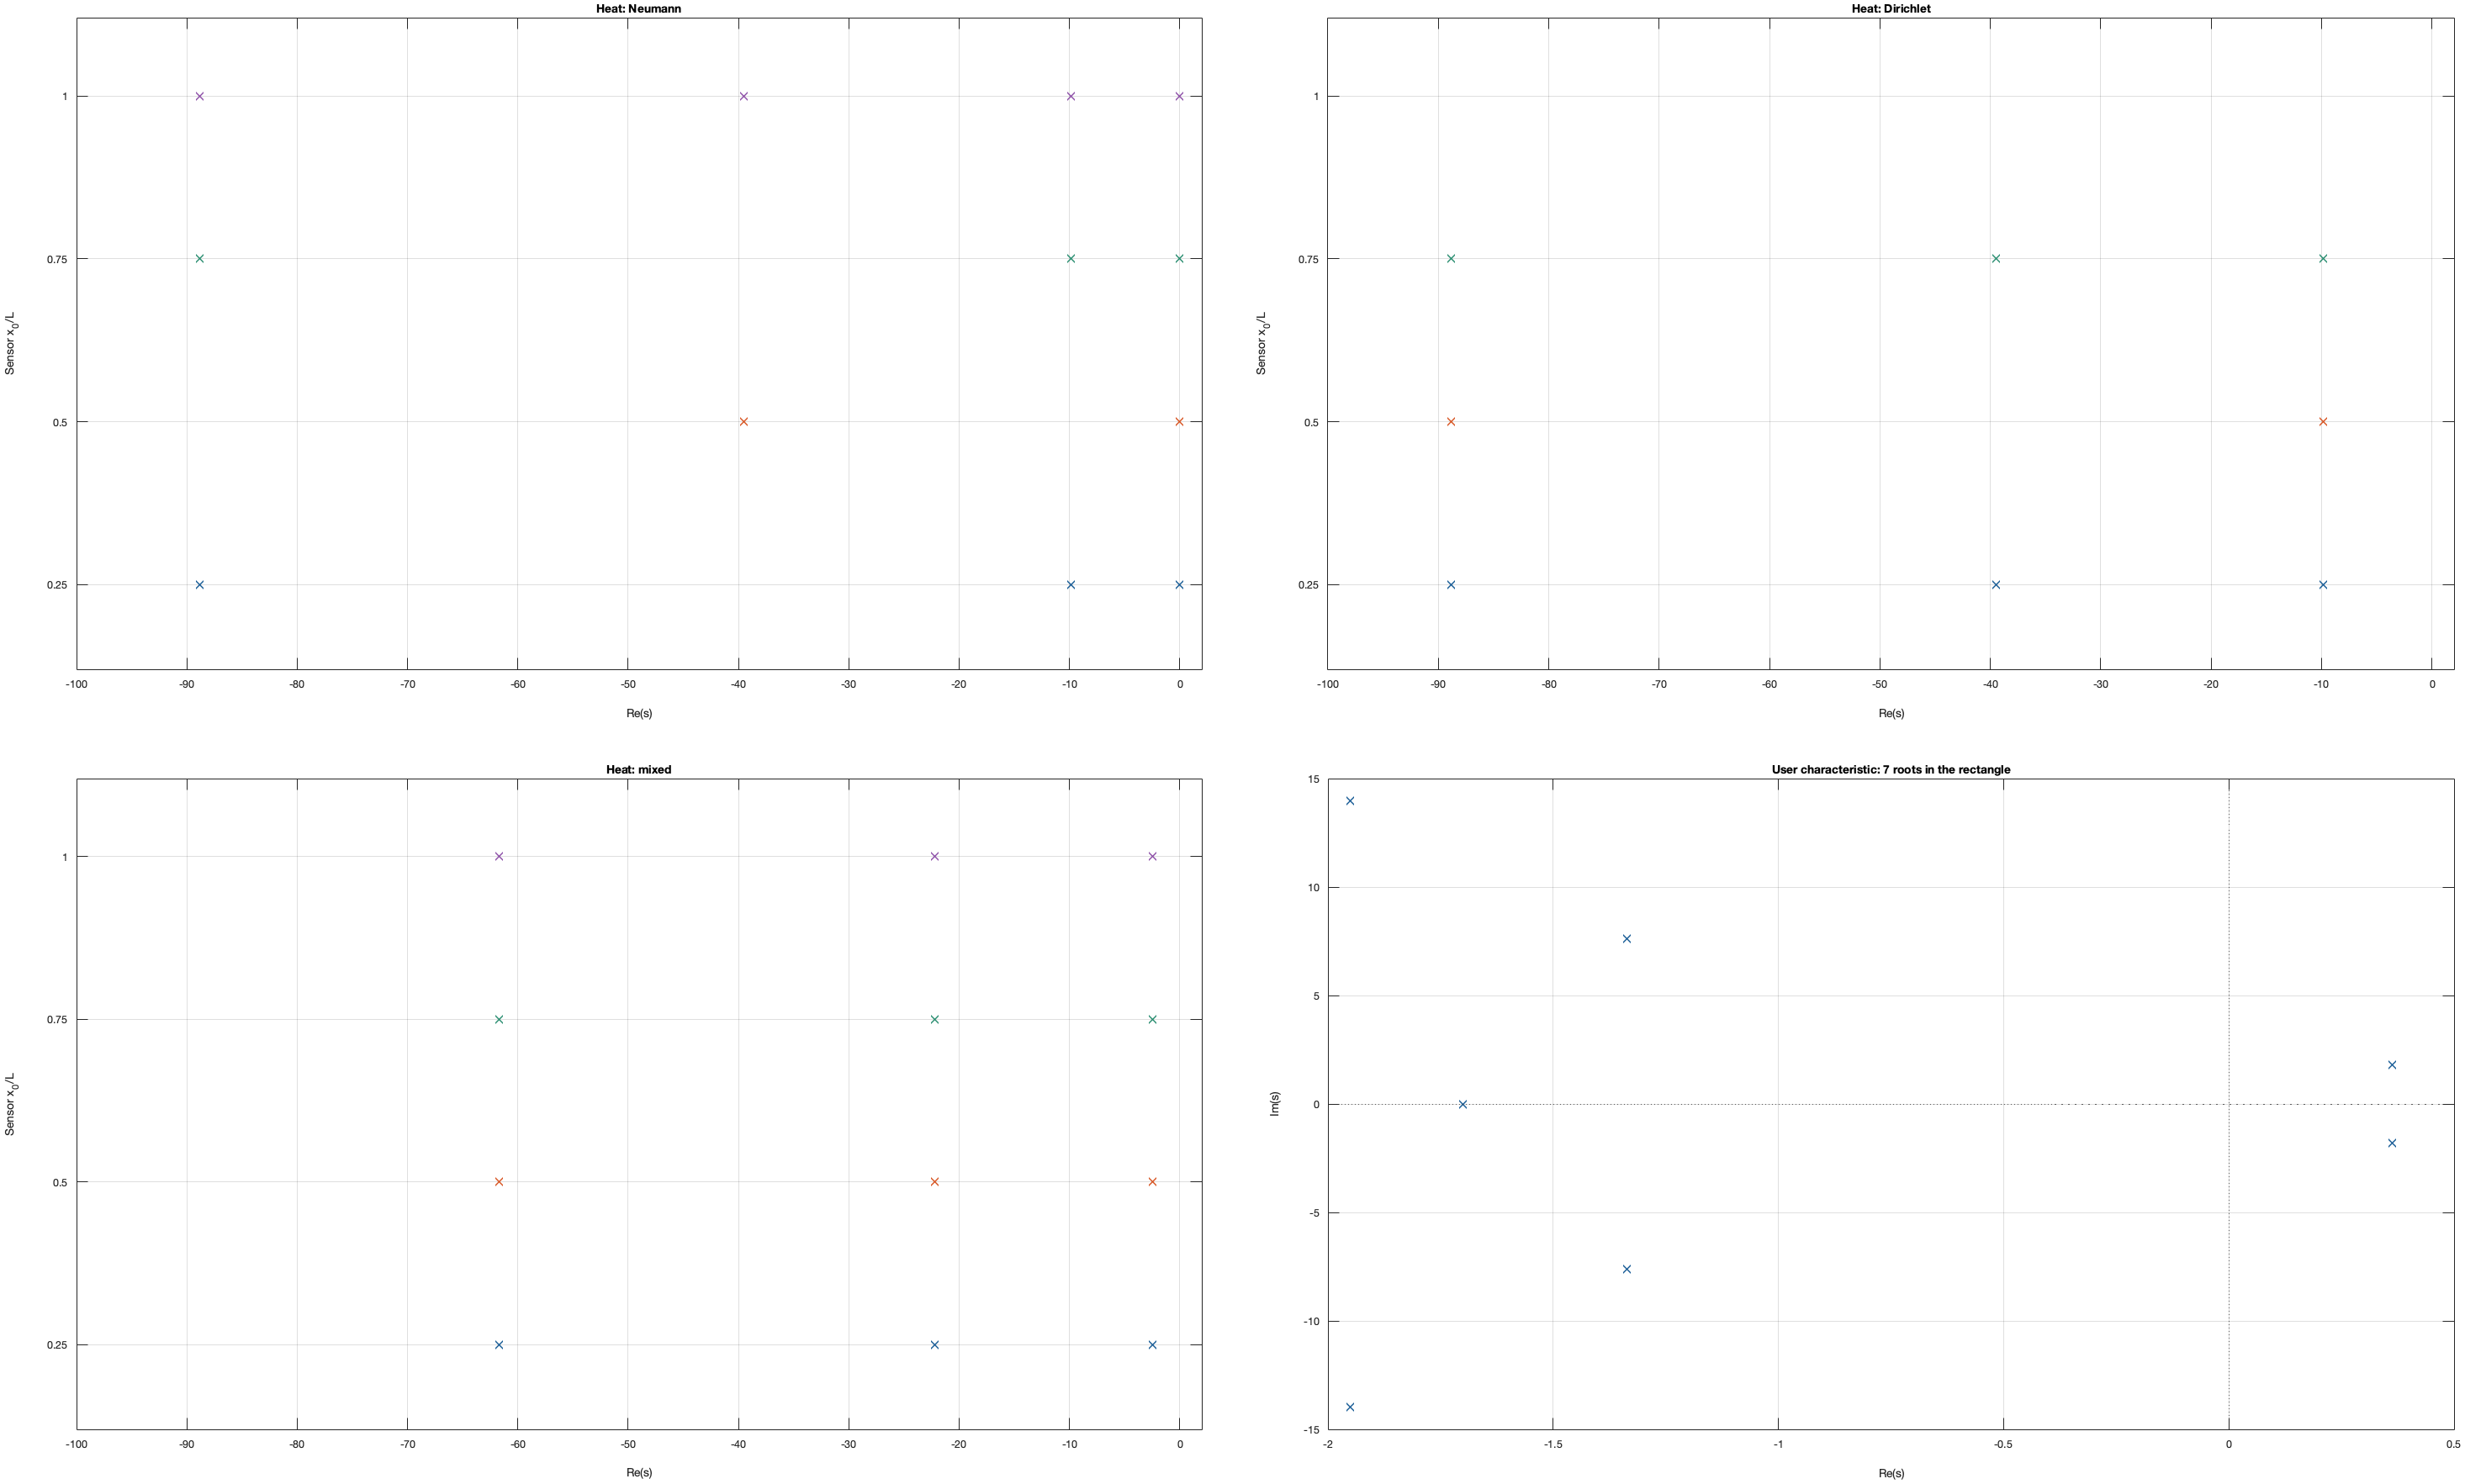
\includegraphics[width=\textwidth]{heat_and_characteristic.png}
\caption{Poles retained for four sensor positions and three boundary
conditions (the Dirichlet row $x_0=1$ is empty because $G=1$). The last
panel shows the characteristic example of Chapter~\ref{ch:quick}.}
\label{fig:heat}
\end{figure}

\section{String and duct}

For the string of Section~2 of the paper, with actuator distribution
$b(x)=1$ on $[0,1/2]$ and $L=c=1$, the modal coefficients are proportional to
$1-\cos(k\pi/2)$, which vanishes for $k$ multiple of 4; those modes are not
poles. The damped model is the output feedback $G/(1+\varepsilon G)$ of the
paper, with $\varepsilon=0.5$, and the removable factor at $s=0$ is
regularized by a series.

For the acoustic duct with constant reflectance $a=0.5$ and $L=c=1$, the
poles lie on the vertical line $\ln(a)/2+\ii k\pi$. With the radiation
impedance of Section~3.4 (Fig.~5 parameters of the paper: $L=3.54$\,m,
$c=341$\,m/s, $\rho=1.20$\,kg/m$^3$, radius $0.101$\,m, sensor at $L/2$), the
reflectance depends on frequency and the poles bend to the left. Its
rational denominator is cleared from $N$ and $D$ together, so that no
artificial poles are introduced (Figure~\ref{fig:waveduct}).

Visible poles of the damped string in the left half-plane do not prove
internal stability of modes hidden from this input/output pair.

\begin{figure}[H]
\centering
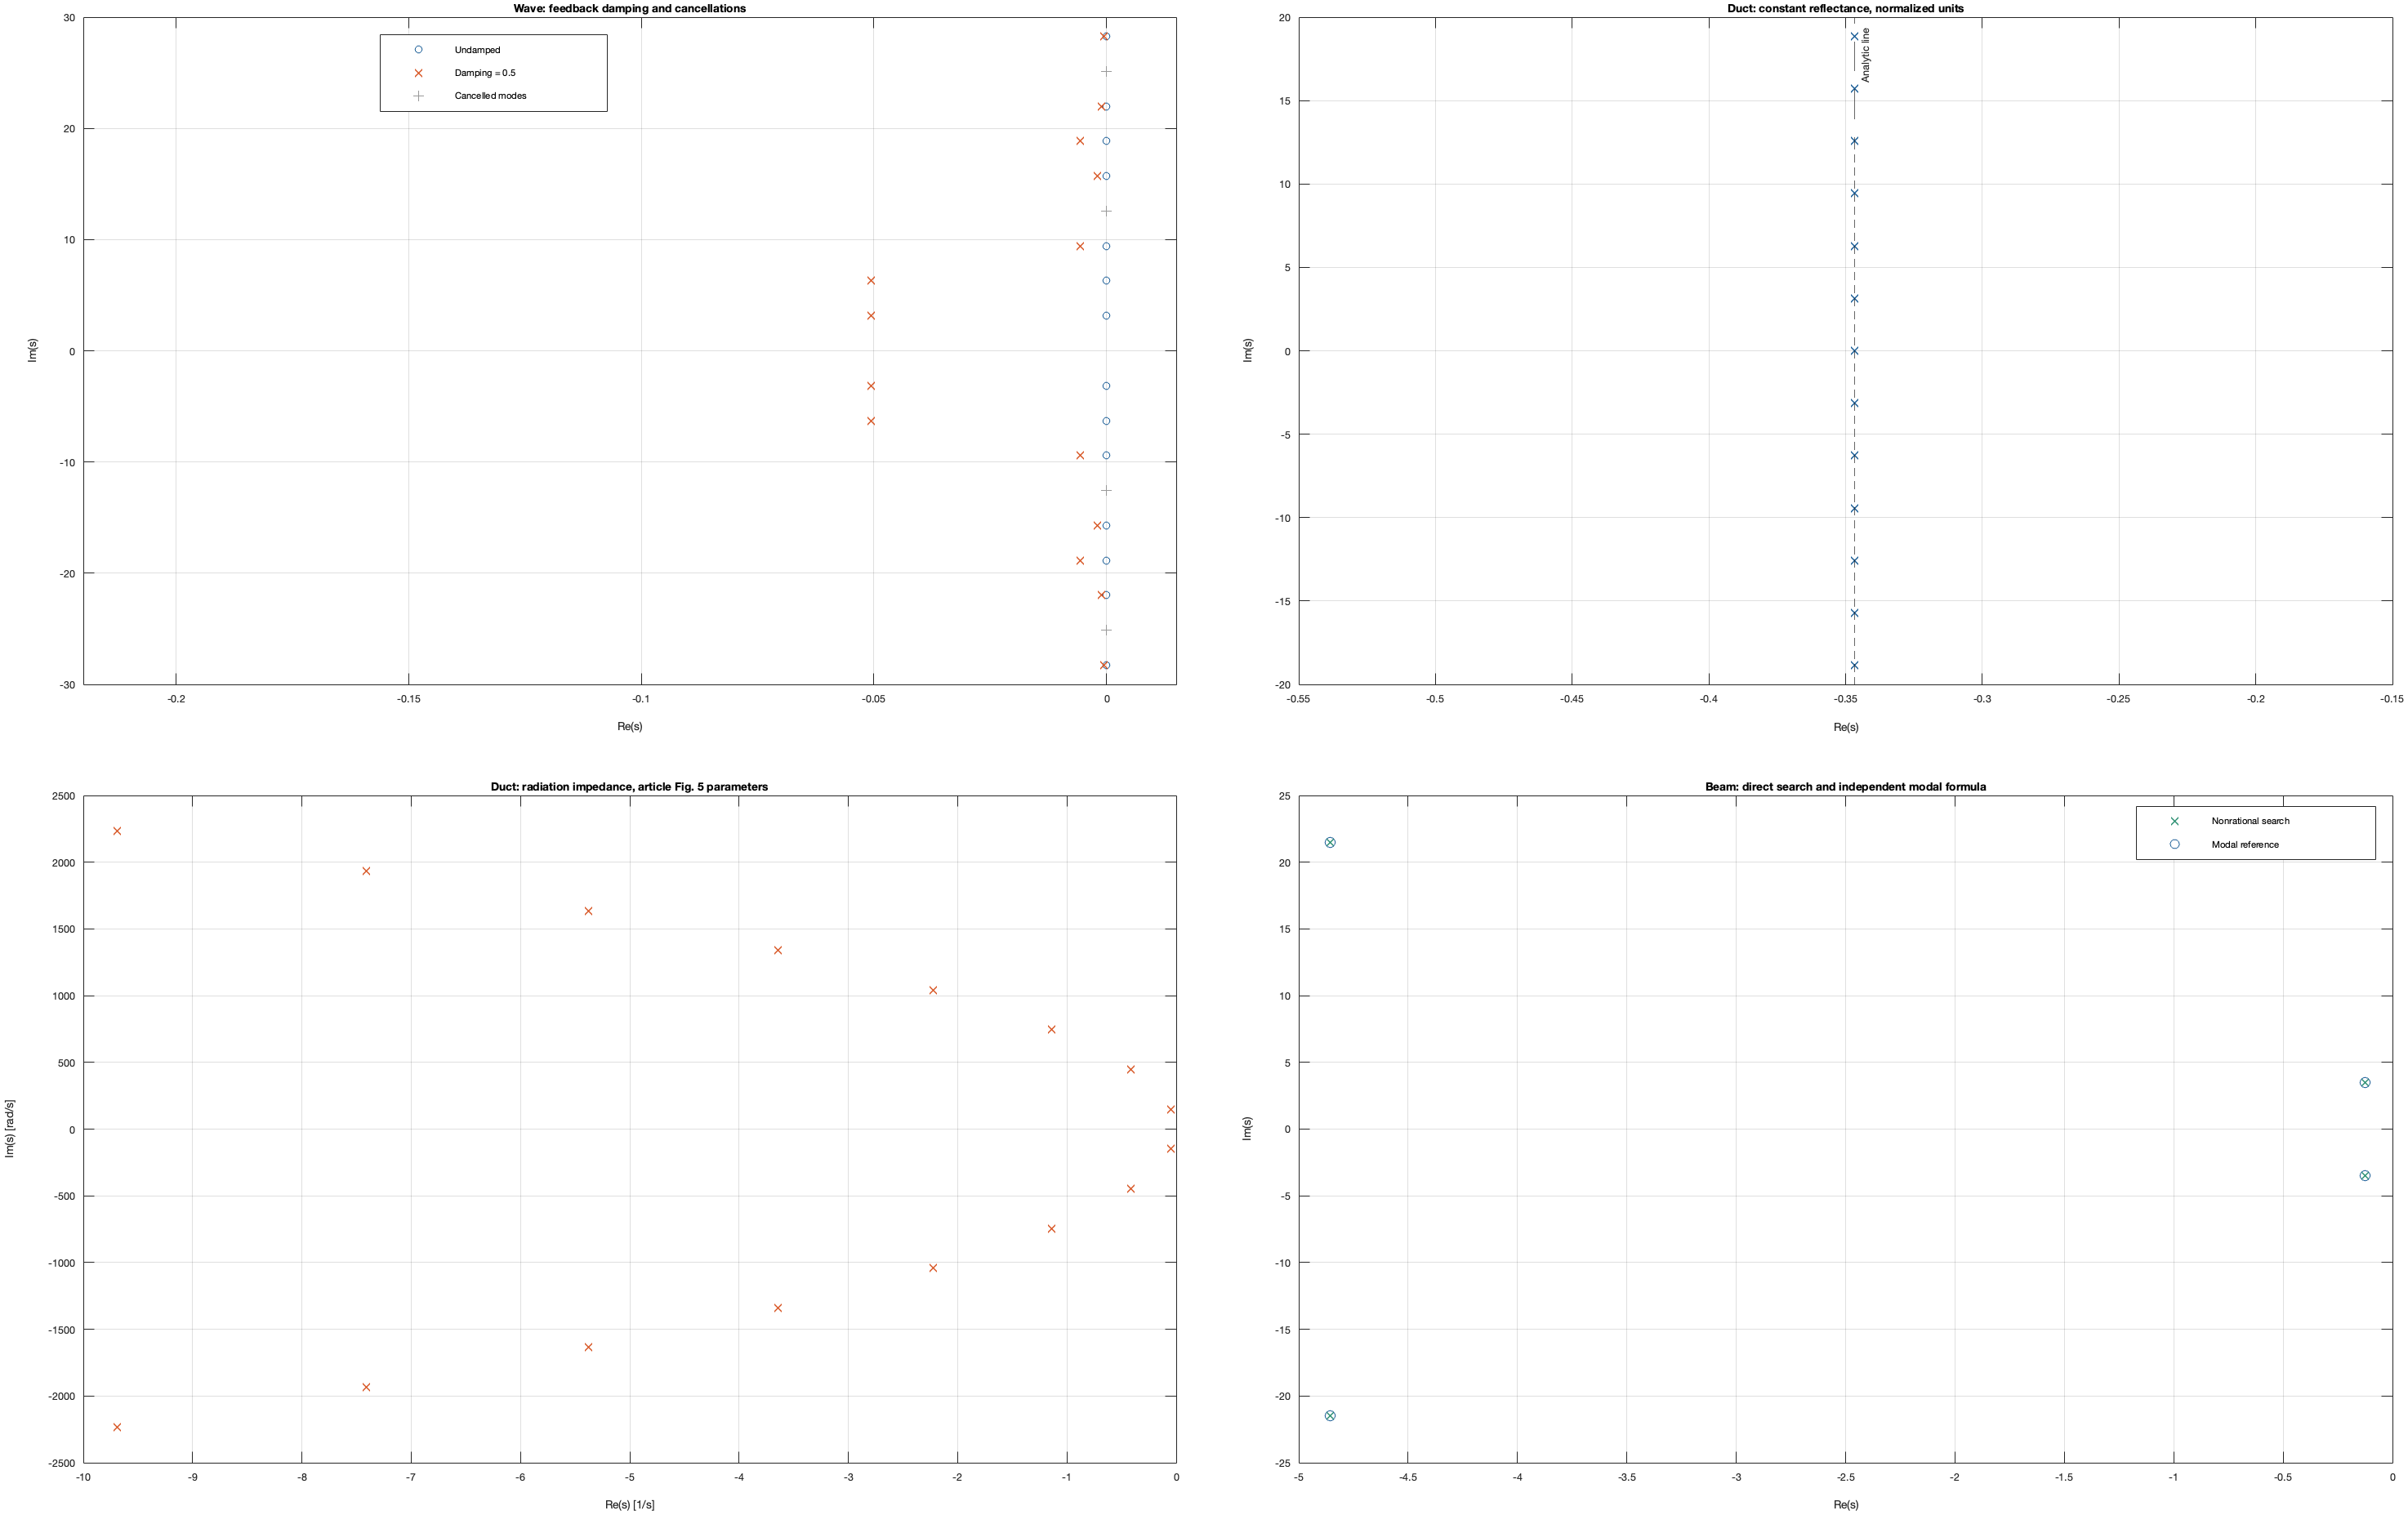
\includegraphics[width=\textwidth]{wave_duct_beam.png}
\caption{String (undamped, damped, and cancelled modes), duct with
constant reflectance and with radiation impedance, and beam poles compared
with an independent modal formula.}
\label{fig:waveduct}
\end{figure}

\section{Kelvin--Voigt beam: an accumulation point}\label{sec:kelvinvoigt}

For the shear-force to tip-velocity transfer function of Section~4.2 of the
paper, with $L=EI=I=1$ and Kelvin--Voigt damping $c_d=0.02$, let
\[
  q(s)=\frac{-s^2}{1+c_ds},\qquad m=q^{1/4},\qquad
  G(s)=\frac{s\,[\cosh m\sin m-\sinh m\cos m]/m^3}{(1+c_ds)[1+\cosh m\cos m]} .
\]
The factors containing $m$ are invariant under $m\mapsto\ii m$, so the choice
of fourth root disappears except at $s=-1/c_d$; the numerator ratio has the
removable value $2/3$ at $m=0$. With the positive roots $\beta_k$ of
$1+\cosh\beta\cos\beta=0$, the poles solve $s^2+c_d\beta_k^4s+\beta_k^4=0$, an
independent reference. In $[-25,2]\times[-160,160]$ the search returns
$-0.12362363\pm3.51384128\ii$ and $-4.85518819\pm21.49292828\ii$, within
$10^{-14}$ of the reference.

As $\beta_k\to\infty$, one branch of these poles converges to $-1/c_d=-50$
(Figure~\ref{fig:accumulation}). Every neighborhood of $-50$ contains
infinitely many poles: $G$ is not meromorphic there, and no finite contour
computation can resolve a region containing that point. The model reports
it in \code{meta.singularities}, and the option \code{Singularities}
rejects any region that contains it.

\begin{figure}[H]
\centering
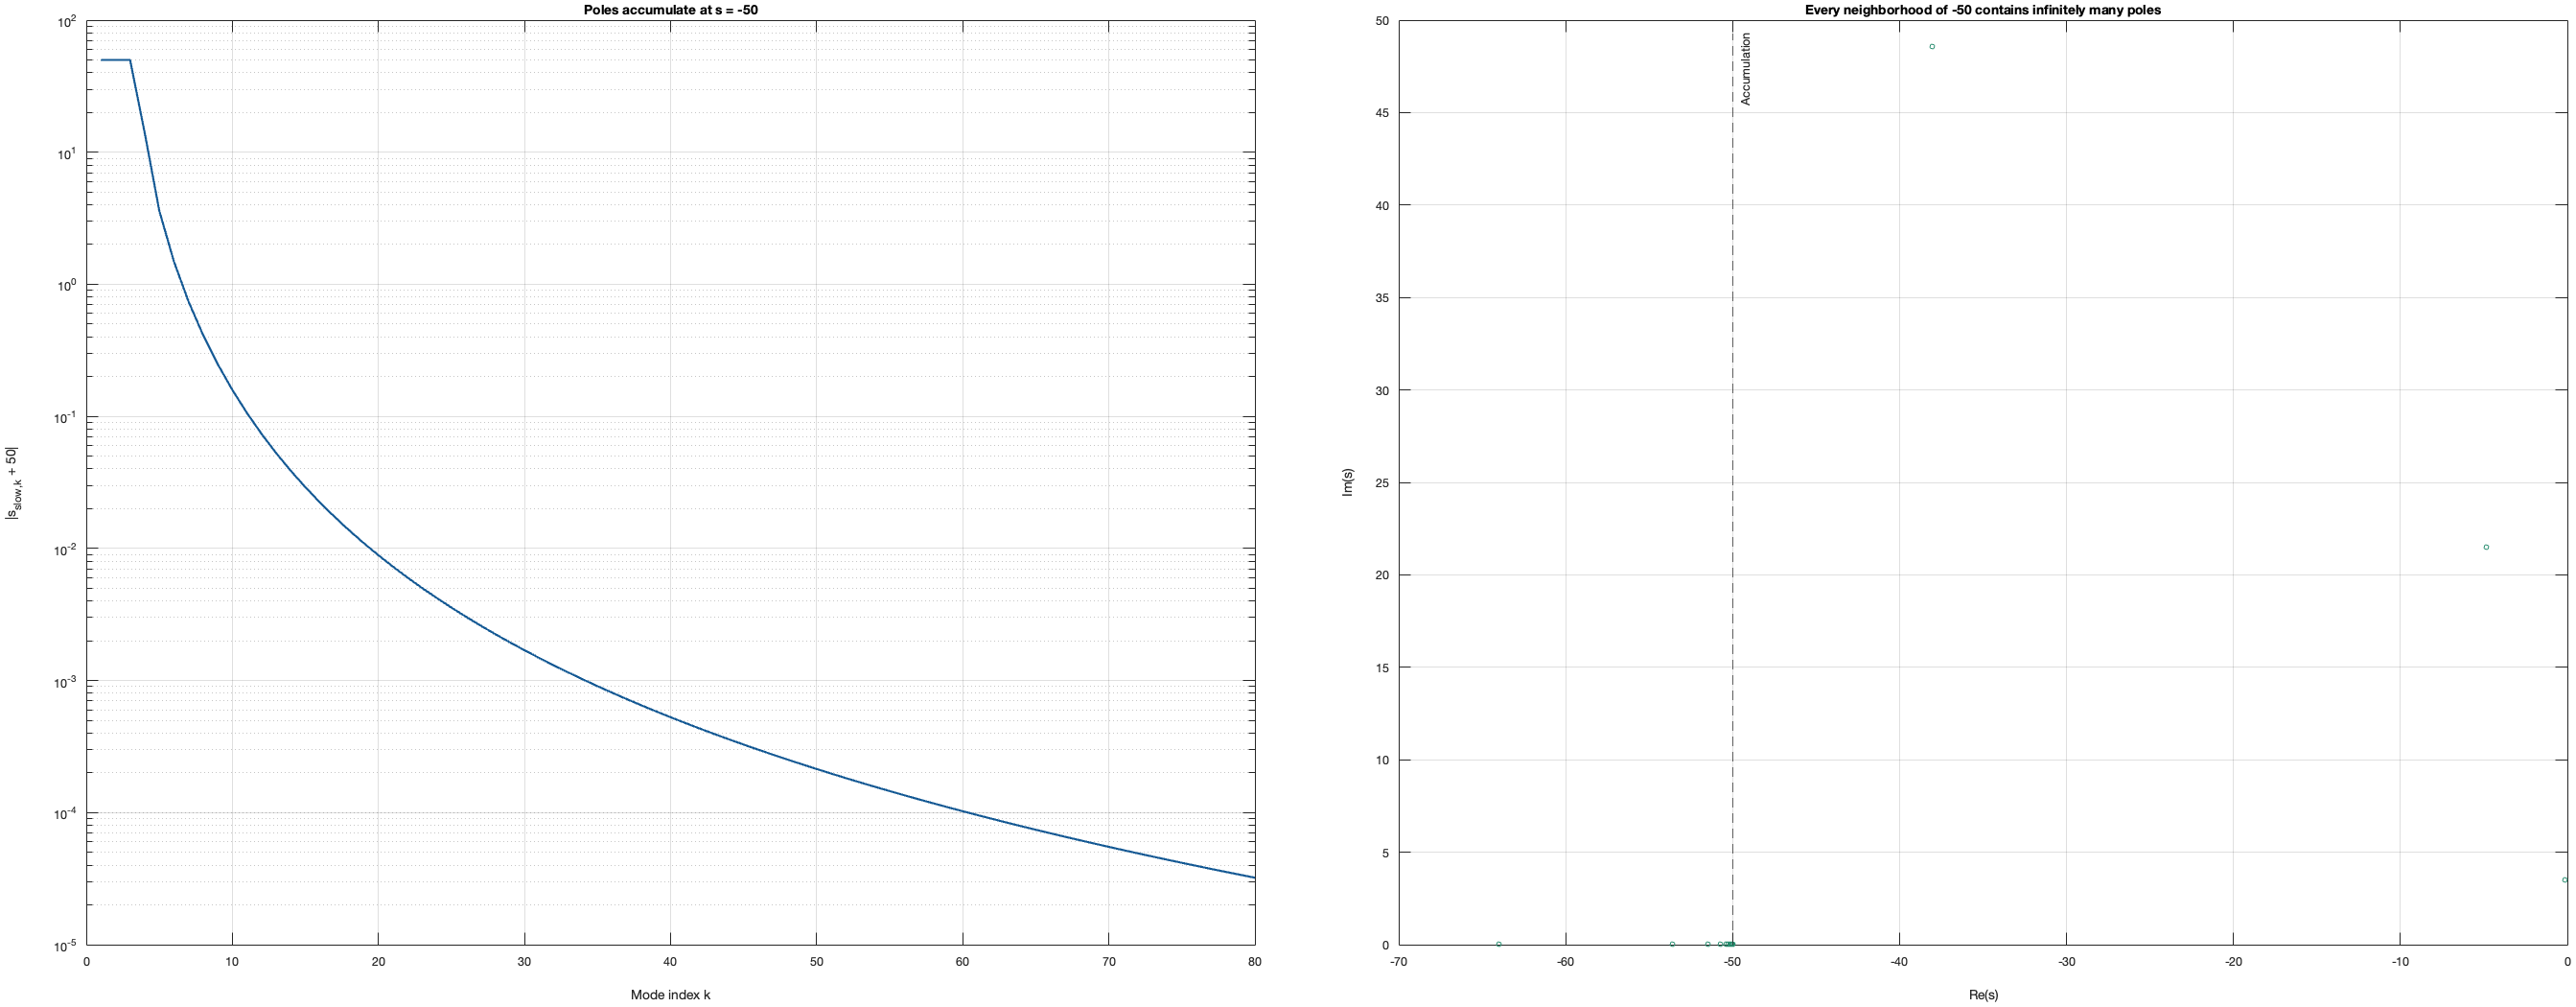
\includegraphics[width=\textwidth]{beam_accumulation.png}
\caption{Modal reference with 80 modes: one branch of poles converges to
$s=-1/c_d=-50$, the other moves to the left.}
\label{fig:accumulation}
\end{figure}

\section{Results}

\begin{table}[H]\centering\small
\caption{Poles in the stated rectangles; ``cancelled'' counts locations.
The reference errors compare with closed-form or modal formulas that are
never used as seeds.}\label{tab:distributed}
\begin{tabular}{lrrrrr}\toprule
Model & $[\Real_{\min},\Real_{\max}]$ & $|\Imag|<$ & Poles & Cancelled & Max. error\\\midrule
Heat, Neumann & $[-100,2]$ & 3 & 2 & 2 & $5\times10^{-14}$\\
Heat, Dirichlet & $[-100,2]$ & 3 & 2 & 1 & $1\times10^{-14}$\\
Heat, mixed & $[-100,2]$ & 3 & 3 & 0 & $7\times10^{-15}$\\
String, undamped & $[-2,1]$ & 30 & 14 & 4 & $3\times10^{-21}$\\
String, $\varepsilon=0.5$ & $[-2,1]$ & 30 & 14 & 4 & ---\\
Duct, constant reflectance & $[-2,1]$ & 20 & 13 & 0 & $2\times10^{-12}$\\
Duct, radiation impedance & $[-400,30]$ & 2500 & 16 & 0 & ---\\
Beam, Kelvin--Voigt & $[-25,2]$ & 160 & 4 & 0 & $7\times10^{-15}$\\
\bottomrule\end{tabular}
\end{table}

For the damped string and the radiating duct there is no independent
closed form; they are verified by the contour counts and the residuals of
the original equations.

\chapter{A beam coupled to an oscillator}\label{ch:beam}

This case study couples a partial differential equation (a beam, with
infinitely many modes) to an ordinary one (a mass-spring-damper), derives an
entire characteristic function and transfer functions, and computes the
poles without modal truncation. The results are validated with an
independent finite-element model.

\begin{figure}[H]
\centering
\begin{tikzpicture}[>=Latex,thick,font=\small,
  spring/.style={decorate,decoration={zigzag,segment length=3.6pt,amplitude=3pt}}]
  \foreach \offset/\labeltext in {0/{(a) Absorber: independent coordinates},8/{(b) Tip mass, grounded spring and damper}} {
    \begin{scope}[xshift=\offset cm]
      \node[anchor=west,font=\small\bfseries] at (-.3,1.1) {\labeltext};
      \fill[pattern=north east lines] (-.4,-.45) rectangle (0,.45);
      \draw[very thick] (0,-.45)--(0,.45);
      \fill[blue!15] (0,-.09) rectangle (4.4,.09);
      \draw (0,-.09)--(4.4,-.09) (0,.09)--(4.4,.09);
      \node at (2.1,.43) {$EI,\ \rho A,\ L$};
      \draw[->,thin] (.25,-.55)--(1.8,-.55) node[right] {$x$};
      \draw[->,blue!70!black] (2.5,-.1)--(2.5,-1.05) node[below] {$w(x,t)$};
    \end{scope}
  }
  % Independent oscillator linked to a massless tip crossbar.
  \fill (4.4,0) circle (2pt);
  \draw (4.4,0)--(4.4,-.4) (3.75,-.4)--(5.05,-.4);
  \draw[spring] (3.75,-.4)--(3.75,-1.75);
  \node[left] at (3.5,-1.05) {$k$};
  \draw (5.05,-.4)--(5.05,-.8);
  \draw (4.81,-1.25)--(4.81,-.8)--(5.29,-.8)--(5.29,-1.25);
  \draw (4.84,-1.02)--(5.26,-1.02) (5.05,-1.02)--(5.05,-1.75);
  \node[right] at (5.35,-1.05) {$c$};
  \draw (3.75,-1.75)--(5.05,-1.75) (4.4,-1.75)--(4.4,-1.98);
  \draw[fill=orange!20] (3.65,-1.98) rectangle (5.15,-2.65);
  \node at (4.4,-2.3) {$m,\ z(t)$};
  \draw[->,blue!70!black] (5.8,.1)--(5.8,-.5) node[right] {$y=w(L,t)$};
  \draw[->,orange!80!black] (5.65,-2.0)--(5.65,-2.85) node[right] {$z$};
  \draw[->,red!70!black] (4.4,.85)--(4.4,.15) node[midway,right] {$f$};
  \node[align=center,font=\footnotesize] at (3,-3.3)
    {Spring and damper act on $z-y$.\\The mass is not connected to the ground.};
  % Rigidly attached point mass, spring and damper connected to ground.
  \begin{scope}[xshift=8cm]
    \draw[fill=orange!20] (3.8,-.3) rectangle (5,.3);
    \node at (4.4,0) {$m$};
    \draw (4.4,-.3)--(4.4,-.55) (3.75,-.55)--(5.05,-.55);
    \draw[spring] (3.75,-.55)--(3.75,-1.9);
    \node[left] at (3.5,-1.2) {$k$};
    \draw (5.05,-.55)--(5.05,-.95);
    \draw (4.81,-1.4)--(4.81,-.95)--(5.29,-.95)--(5.29,-1.4);
    \draw (4.84,-1.17)--(5.26,-1.17) (5.05,-1.17)--(5.05,-1.9);
    \node[right] at (5.35,-1.2) {$c$};
    \draw (3.2,-1.9)--(5.6,-1.9);
    \fill[pattern=north east lines] (3.2,-2.13) rectangle (5.6,-1.9);
    \draw[->,blue!70!black] (5.8,.1)--(5.8,-.65) node[right] {$y=z$};
    \node[align=center,font=\footnotesize] at (3,-3.3)
      {Spring and damper act on $y$.\\The mass moves rigidly with the tip.};
  \end{scope}
\end{tikzpicture}

\caption{The two topologies. The connection transmits transverse force but
no moment; displacements are positive downwards.}
\label{fig:schematic}
\end{figure}

\section{Model}

A uniform Euler--Bernoulli beam of length $L$, bending stiffness $EI$ and
mass per length $\mu_b=\rho A$ is clamped at $x=0$. In topology (a), a mass
$m$ with displacement $z(t)$ is connected to the tip displacement
$y(t)=w(L,t)$ by a spring $k$ and a damper $c$ in parallel; the mass is not
grounded (a tuned-mass absorber). The beam is elastic; all dissipation is in
$c$. Shear deformation, rotary inertia and gravity (already balanced) are
neglected:
\begin{gather}
  \mu_bw_{tt}+EIw_{xxxx}=0,\quad 0<x<L,\qquad w(0,t)=w_x(0,t)=0,\\
  EIw_{xx}(L,t)=0,\qquad -EIw_{xxx}(L,t)=F(t)+f(t),\\
  f=k(z-y)+c(\dot z-\dot y),\qquad m\ddot z+c(\dot z-\dot y)+k(z-y)=u(t),
\end{gather}
where $f$ is the force of the connection on the beam and $F$, $u$ are
external forces at the tip and on the mass.

\section{The bare-beam receptance}

With $w=W(x)e^{st}$ and $\theta^4=q=-\mu_bL^4s^2/EI$, the clamped solution
is $W(x)=a[\cosh bx-\cos bx]+d[\sinh bx-\sin bx]$, $b=\theta/L$. The
zero-moment condition fixes $d/a$, and the shear condition gives the tip
receptance
\[
  H_b(s)=\frac{y}{f}=\frac{L^3}{EI}\frac{A(q)}{B(q)},\quad
  A(q)=\frac{\cosh\theta\sin\theta-\sinh\theta\cos\theta}{\theta^3},\quad
  B(q)=1+\cosh\theta\cos\theta .
\]
$A$ and $B$ are entire in $q$: they are invariant under $\theta\mapsto\ii\theta$.
Near $q=0$, $A(q)=\tfrac23-\tfrac q{315}+\tfrac{q^2}{623700}-\tfrac{q^3}{5108103000}+\cdots$
and $B(0)=2$, so $H_b(0)=L^3/(3EI)$, the static compliance of a cantilever.
Write $H_b=N_b/D_b$ with $N_b=(L^3/EI)A$, $D_b=B$.

\section{Characteristic function and transfer functions}

With $Z(s)=k+cs$ the Laplace-domain equations are
\[
  \begin{bmatrix}D_b+N_bZ & -N_bZ\\ -Z & ms^2+Z\end{bmatrix}
  \begin{bmatrix}y\\ z\end{bmatrix}=
  \begin{bmatrix}N_bF\\ u\end{bmatrix},
\]
whose determinant is the entire characteristic function
\begin{equation}
  \Delta(s)=D_b(s)(ms^2+cs+k)+N_b(s)\,ms^2(cs+k) .
  \label{eq:beamdelta}
\end{equation}
The coupled poles are not the union of the beam and oscillator poles, and
$1+H_bZ_{\mathrm{eff}}$, with $Z_{\mathrm{eff}}=ms^2(cs+k)/(ms^2+cs+k)$, is
not entire; clearing its denominators gives~\eqref{eq:beamdelta}. The
transfer functions are
\[
  \frac yF=\frac{N_b(ms^2+Z)}{\Delta},\qquad
  \frac yu=\frac{N_bZ}{\Delta},\qquad
  \frac zu=\frac{D_b+N_bZ}{\Delta}.
\]
With zero inputs, the energy
$E=\tfrac12\int_0^L(\mu_bw_t^2+EIw_{xx}^2)\,dx+\tfrac12m\dot z^2+\tfrac12k(z-y)^2$
satisfies $\dot E=-c(\dot z-\dot y)^2\le0$, which confirms the sign
conventions and excludes growing modes for positive parameters. In topology
(b) the mass moves with the tip and $\Delta_{\mathrm{tip}}=D_b+N_b(ms^2+cs+k)$;
it is a different system, with potential energy $ky^2/2$.

\section{Implementation}

With $\tau=\sqrt{\mu_bL^4/EI}$, $\lambda=\tau s$, $\mu=m/(\mu_bL)$,
$\kappa=kL^3/EI$ and $\gamma=cL^3/(EI\tau)$, the function evaluated is
$\Delta=B(-\lambda^2)(\mu\lambda^2+\gamma\lambda+\kappa)+A(-\lambda^2)\mu\lambda^2(\gamma\lambda+\kappa)$,
equal to~\eqref{eq:beamdelta} times $L^3/EI$. In normalized units the
complete computation needs only function handles:
\begin{lstlisting}
m = 0.1;  k = 1.2362363368;  c = 0.05;      % L = EI = rho*A = 1
beta = @(s) (-s.^2).^(1/4);
Nb = @beam_numerator;                        % series near 0, see text
Db = @(s) 1 + cosh(beta(s)).*cos(beta(s));
Zc = @(s) k + c*s;
N = @(s) Nb(s).*(m*s.^2 + Zc(s));
D = @(s) Db(s).*(m*s.^2 + Zc(s)) + Nb(s).*m.*s.^2.*Zc(s);
[p, info] = cpoles(ndpair(N, D), [-60 1 -150 150], 'AssumeAnalytic', true);
\end{lstlisting}
The full script is \path{examples/coupled_beam/beam_direct_nd.m}; the
helper \path{examples/models/coupled_beam_model.m} builds the dimensional
model and the three transfer functions.

\section{Reference case and parameter studies}

The reference case uses $m=0.1$, $k=m\,\omega_{b1}^2=\BaselineStiffness$ with
the first bare-beam frequency $\omega_{b1}=\FirstBareFrequency$, and $c=0.05$.
The ten poles in $[-60,1]\times[-150,150]$ are (upper half-plane):
\begin{center}\small\BaselinePoleTable\end{center}
For $c=0$ the two lowest frequencies are $2.5703$ and $4.7801$: the coupling
splits the original resonance; in the first mode the mass follows the tip,
in the second it moves against it (Figure~\ref{fig:modes}).

\begin{figure}[H]
\centering
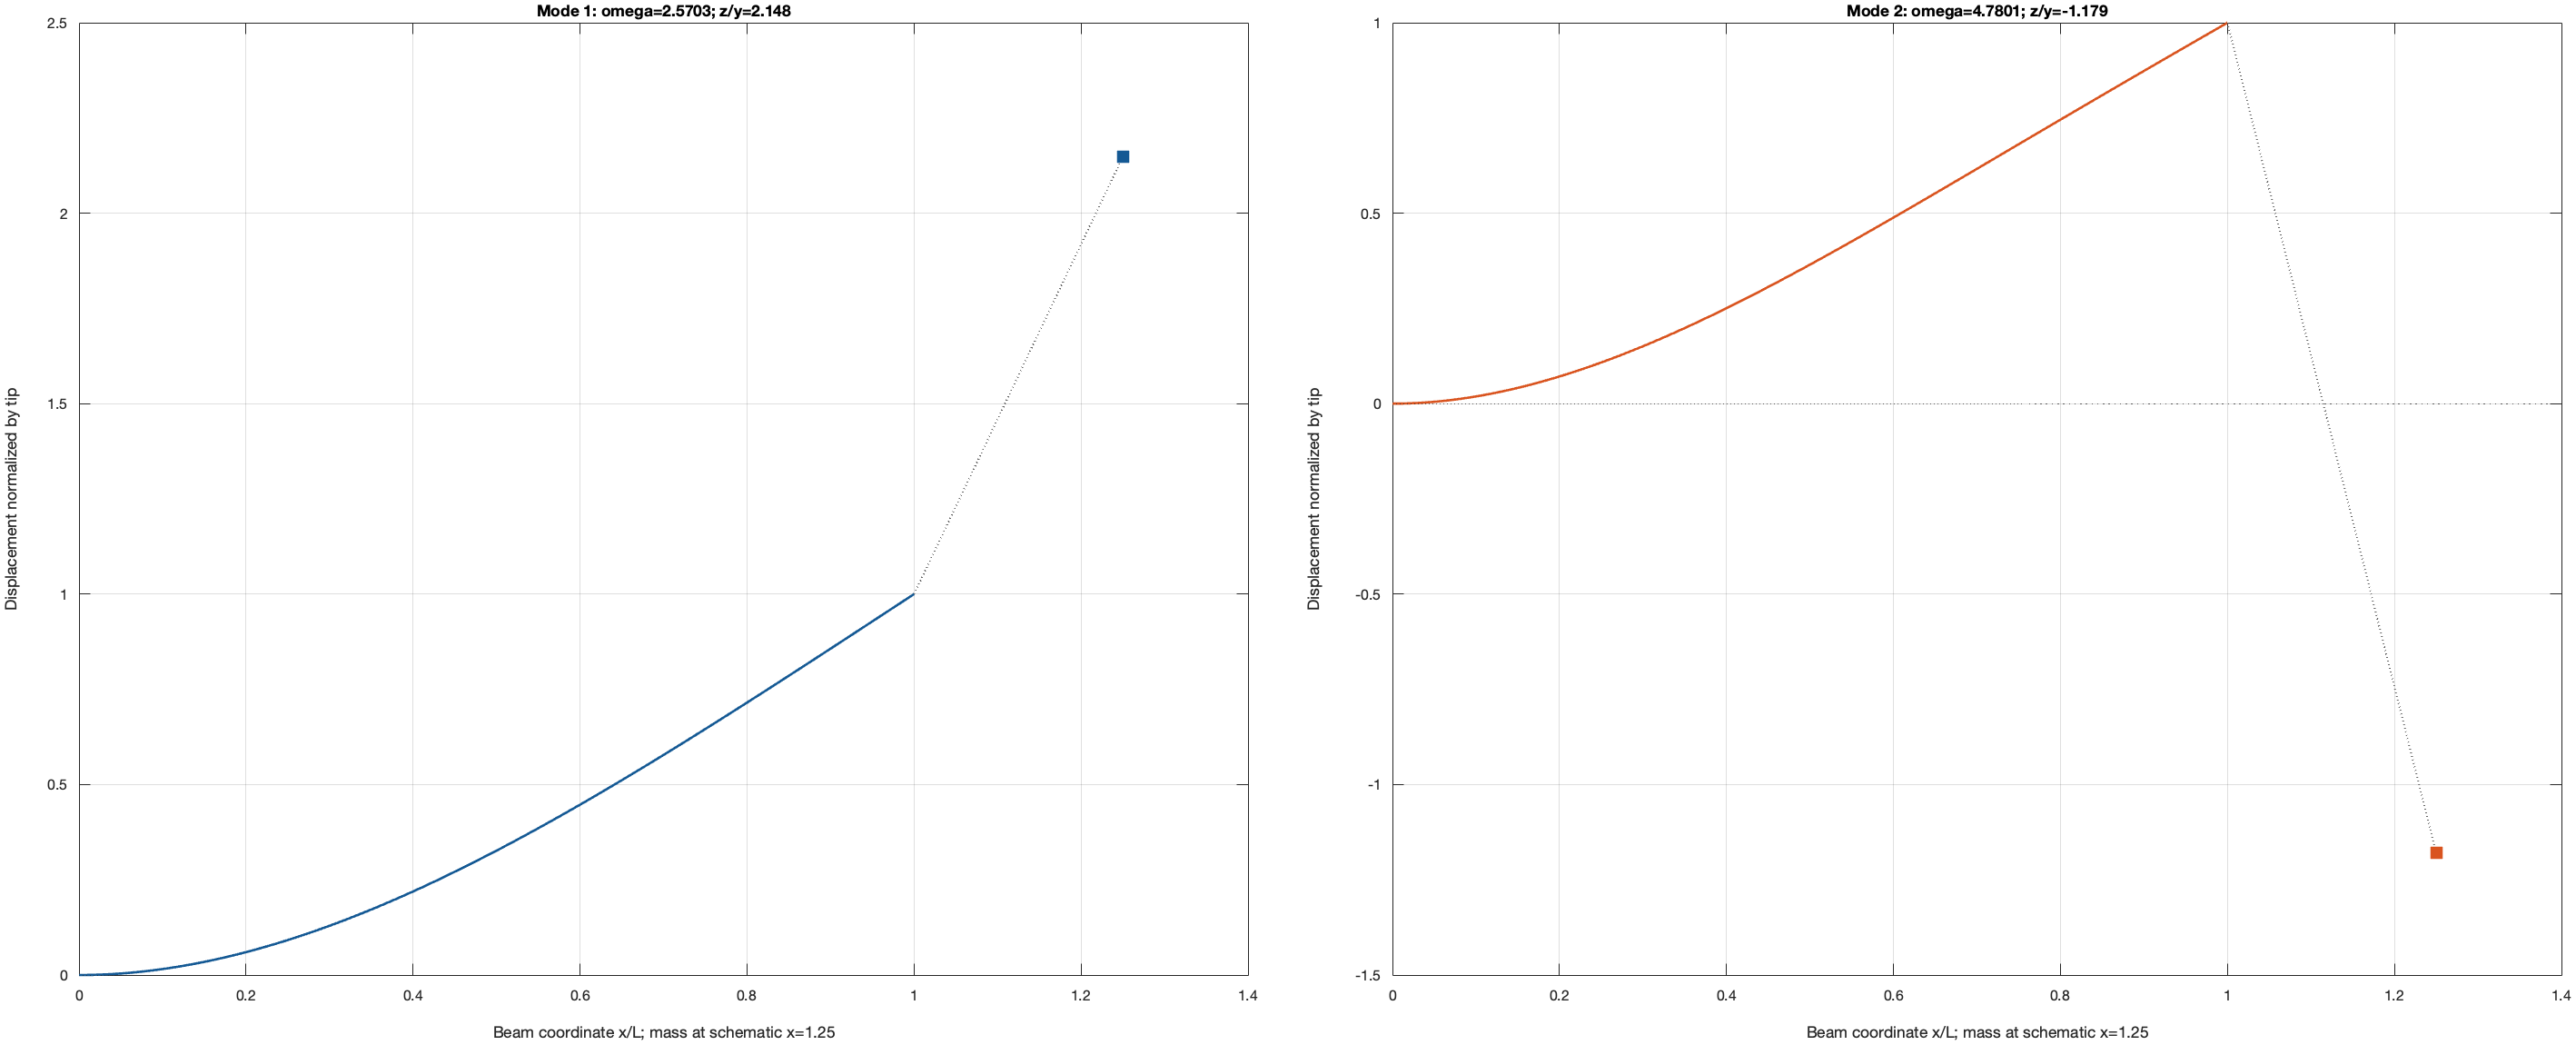
\includegraphics[width=\textwidth]{coupled_modes.png}
\caption{Conservative coupled modes from the exact spatial solution,
normalized by the tip displacement.}
\label{fig:modes}
\end{figure}

One parameter at a time was varied: $m\in[0.02,0.5]$ (25 values),
$k\in[0.05,5]$ (36 values) and $c\in[0,1.5]$ (43 values). Every one of the
104 cases has ten poles in the window, each found with a fresh contour
count (previous poles were only seeds).

\begin{figure}[H]
\centering
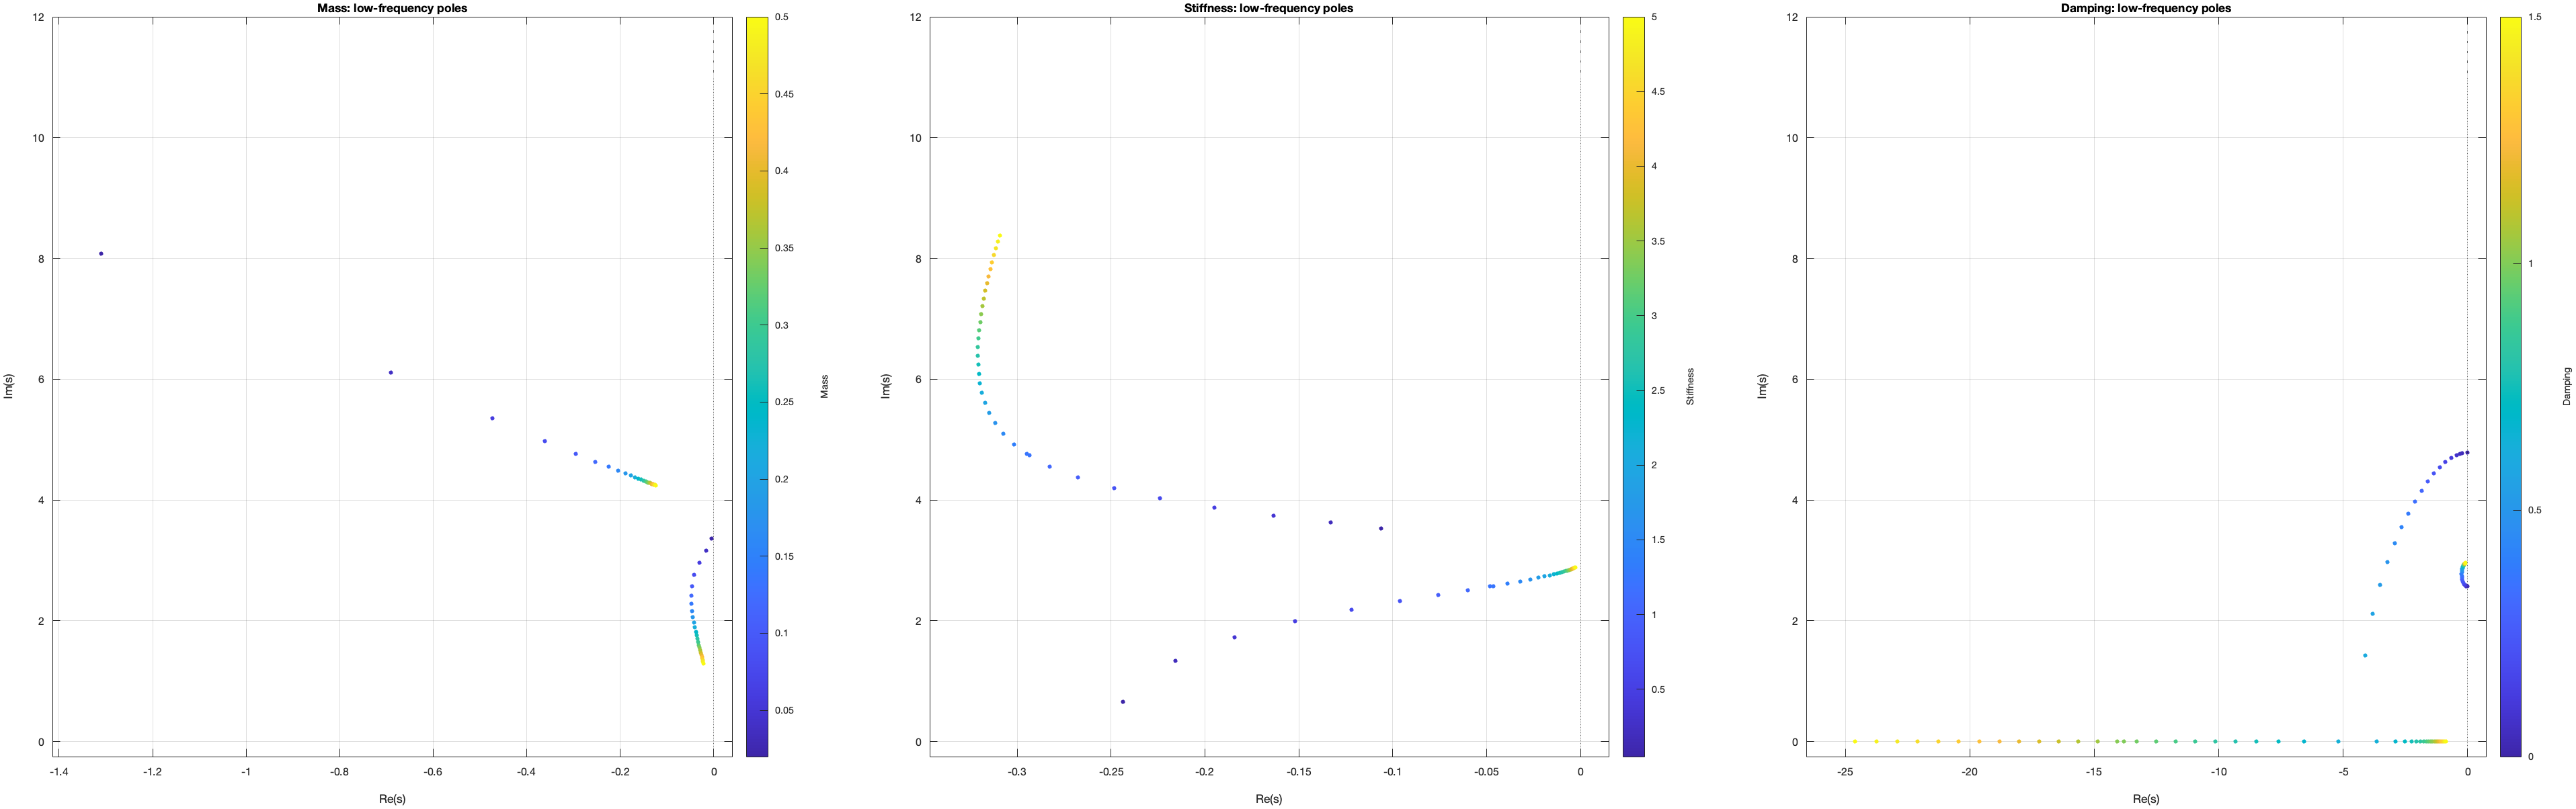
\includegraphics[width=\textwidth]{pole_sweeps.png}
\caption{Low-frequency poles as the mass, the stiffness and the damping vary.}
\label{fig:sweeps}
\end{figure}

\begin{center}\small\DampingPoleTable\end{center}

Increasing $c$ can make the second pair real. Among the sampled values the
rightmost pole is leftmost at $c=\BestDamping$ (abscissa $\BestAlpha$); at
$c=1.5$ the dominant pair returns to $-0.0840\pm2.9549\ii$. Damping in the
connection restrains the very relative motion it dissipates, so more
damping is not always better. This is a statement about the sampled values
and the stated window, not a global optimum.

\begin{figure}[H]
\centering
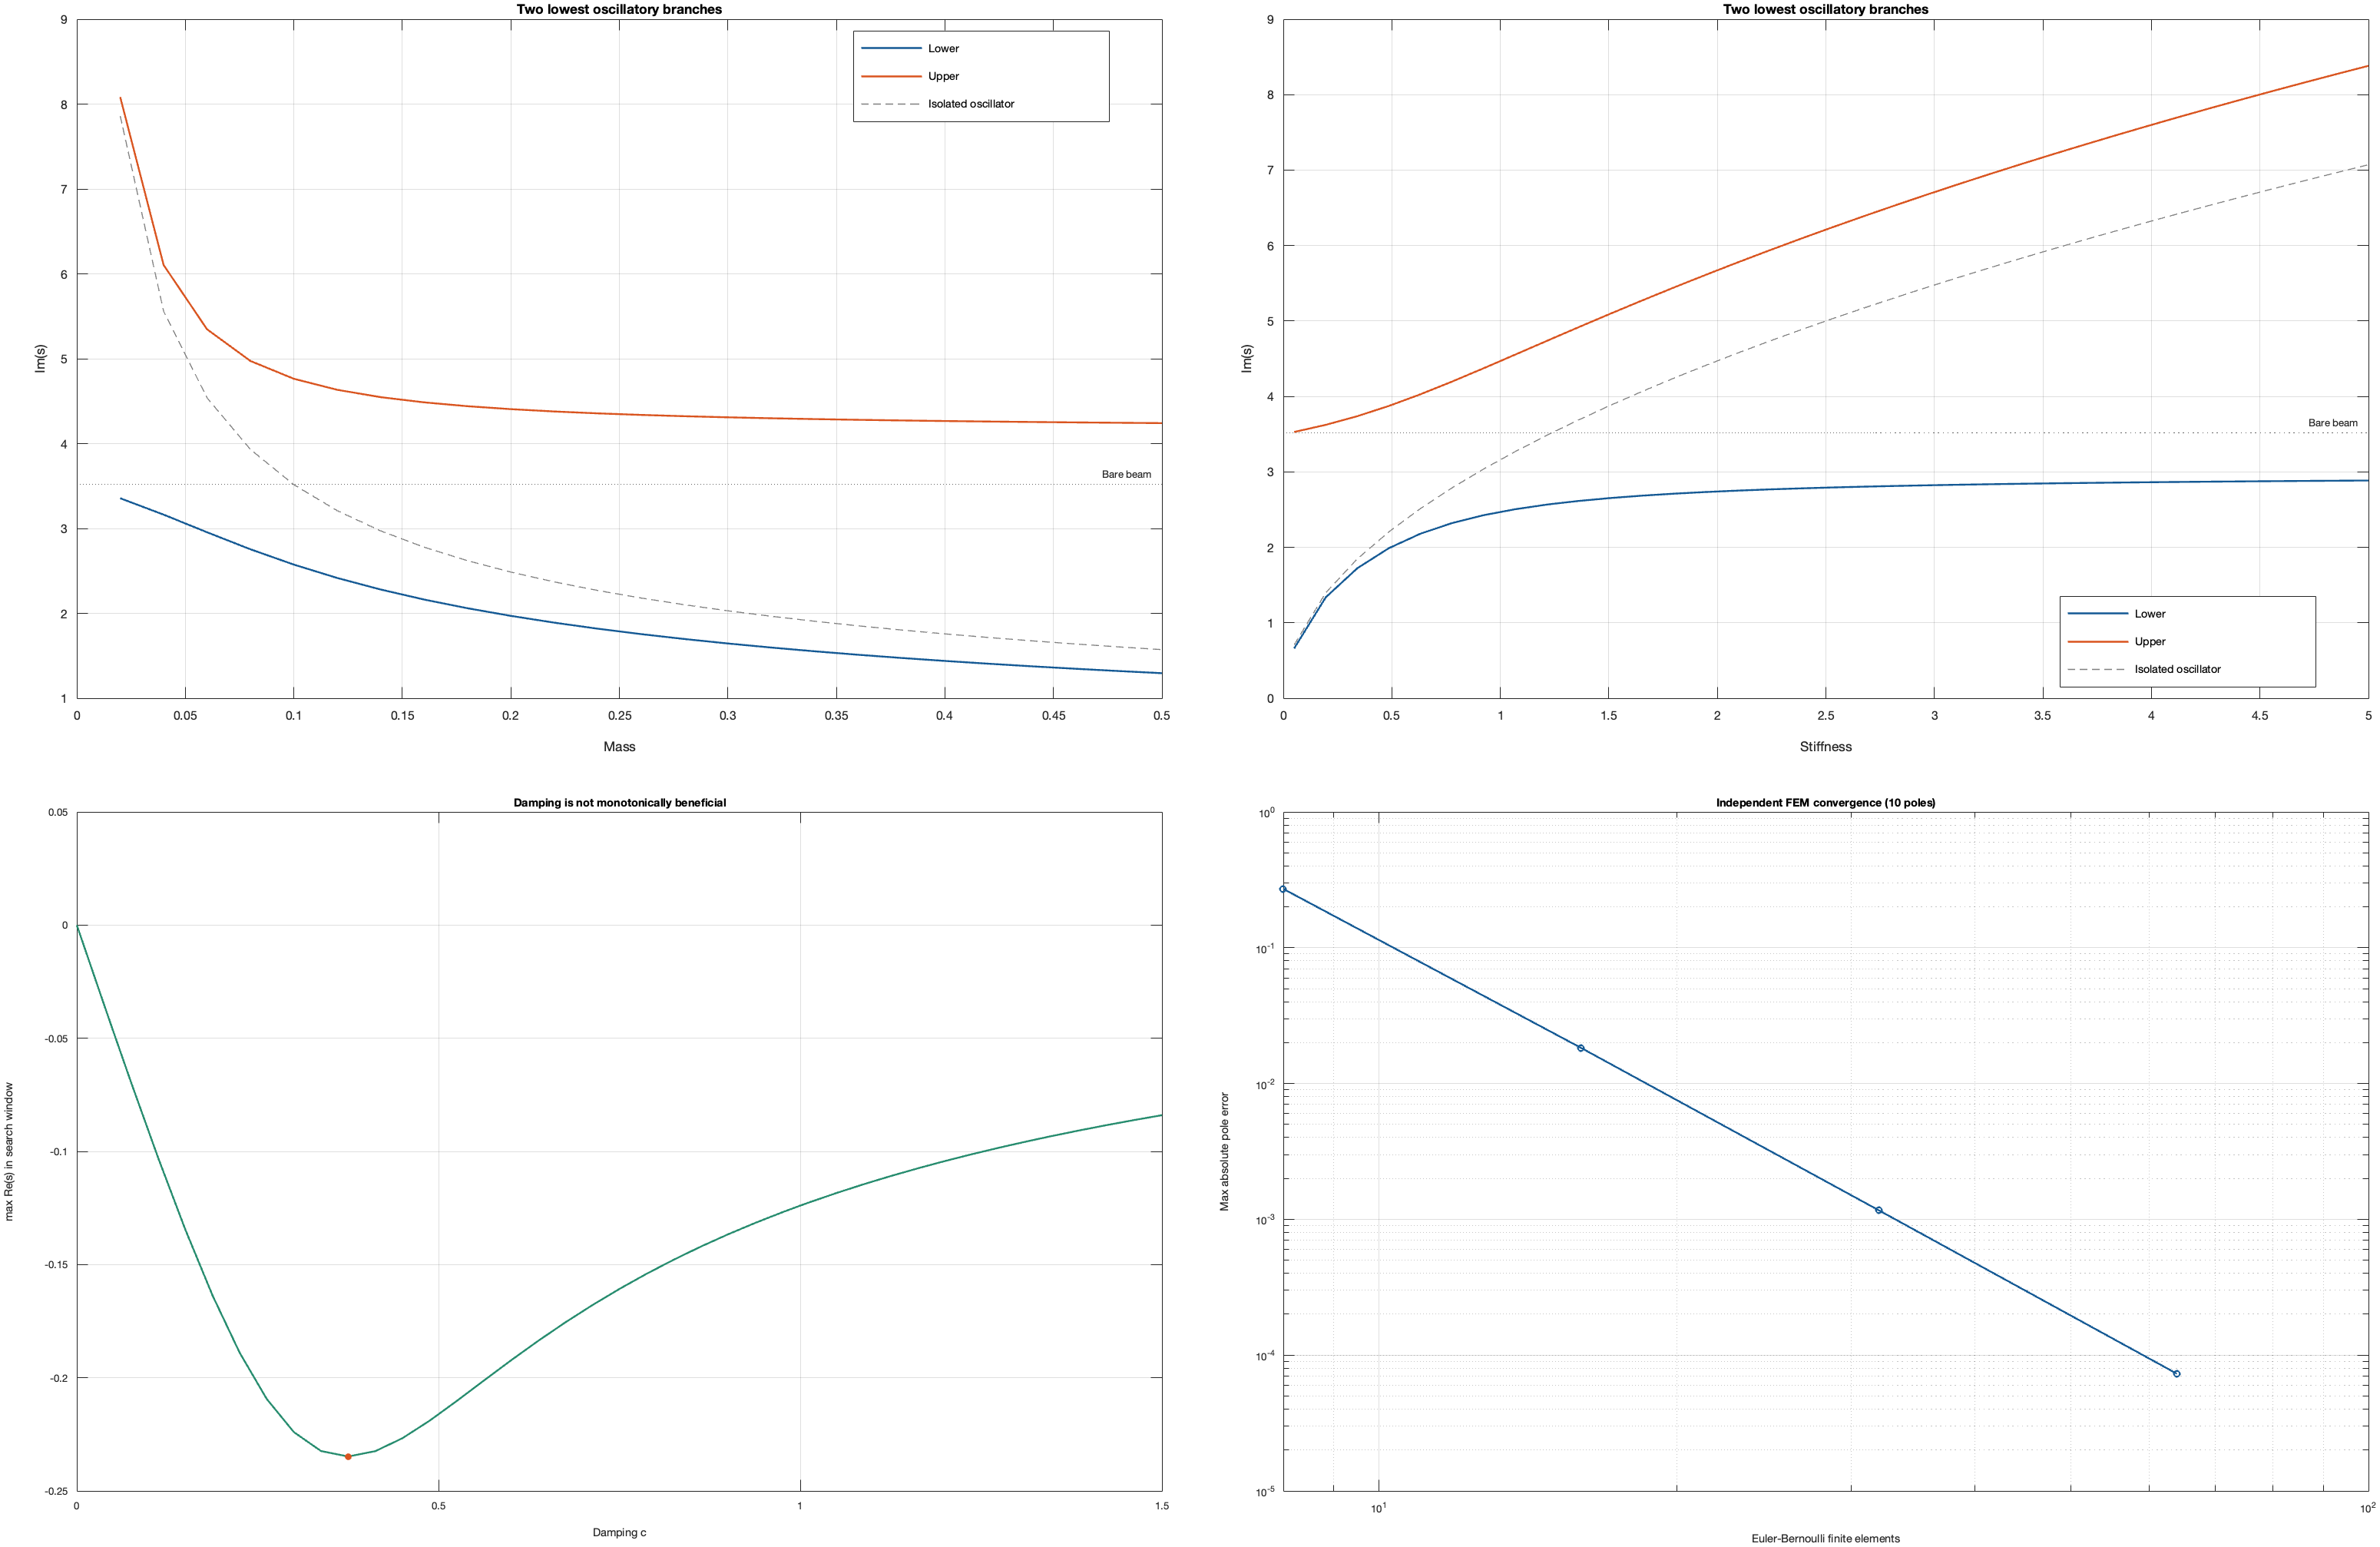
\includegraphics[width=\textwidth]{trends_and_validation.png}
\caption{Lowest branches versus mass and stiffness, window abscissa versus
damping, and convergence of the finite-element model.}
\label{fig:trends}
\end{figure}

\section{Independent validation}\label{sec:beamvalidation}

A cubic-Hermite finite-element model with consistent mass matrix and an
extra degree of freedom for the absorber mass (\code{coupled\_beam\_fem.m})
is solved as a quadratic eigenvalue problem, without using any result of the
nonrational solver. The largest error among the ten reference poles
decreases with the mesh:
\begin{center}\small\FEMTable\end{center}
Further checks: the static compliance $H_b(0)=1/3$; invariance of the
dimensionless characteristic function under dimensional rescaling; the
bare-beam limit; and the decoupled limit $k=c=0$, where the characteristic
function has a double root at $0$ (the free mass) that is \emph{not} a pole
of the tip transfer function $y/F$ --- a hidden mode. Enlarging the window
to $[-90,1]\times[-300,300]$ at three damping values leaves the rightmost
pole unchanged. The beam is elastic and has no finite accumulation point,
unlike the Kelvin--Voigt beam of Section~\ref{sec:kelvinvoigt}.

\chapter{Validation and limitations}\label{ch:validation}

\section{Test suite}

The test suite (\code{buildtool test} and \code{buildtool docs}) has four
layers.
\begin{description}
  \item[Unit tests] of the public interface: agreement of \code{croots},
    \code{cpoles}, \code{czeros} and \code{cpzmap} with the core solver;
    polynomial input against \code{roots}; cancellations; warnings for
    exploratory and incomplete searches; input errors.
  \item[Regression tests] of the numerical behavior: a triple root; three
    roots under scalings of $10^{\pm100}$; a function without zeros;
    boundary roots and exhausted budgets that must not be reported as
    complete; heat, string and duct poles against closed forms; total and
    partial cancellation; an opaque handle with $Z-P=0$; symbolic and LTI
    input; the delay tools (closed-form critical delay, delay-independent
    stability, Padé predictions, bound-based counts); the coupled beam
    (static compliance, limits, scaling, finite-element convergence).
  \item[Baseline] results of the research code from which the toolbox was
    extracted must be reproduced within a relative tolerance of $10^{-9}$.
  \item[Documentation tests] execute every MATLAB block of the README and
    of the Markdown documentation, the quick-start scripts, and check that
    code shown in tutorials is identical to the example files.
\end{description}

\section{Independent references in the studies}

The studies of Chapters~\ref{ch:delay}--\ref{ch:beam} compare the solver
with closed forms (critical delay of P1; heat, string and duct spectra),
modal formulas (Kelvin--Voigt beam), the direct critical-delay method and
bound-based counts (stability maps), time-domain integration with
\code{dde23}, and a finite-element model (coupled beam). The references are
never used as Newton seeds.

\section{Limitations}

\begin{itemize}
  \item Scalar functions only; matrix and MIMO problems are not treated.
  \item Rectangular regions only; roots outside the rectangle are not
        considered, and infinite spectra are not enumerated.
  \item Completeness is a numerical check under the analyticity assumption
        (Section~\ref{sec:contract}), not an interval-arithmetic proof.
  \item Analyticity of function handles, and the location of branch and
        accumulation points, must be established by the user.
  \item Roots closer than the confirmation resolution are reported as
        clusters; near pole-zero pairs may be reported as cancelled.
  \item The time-delay tools assume one constant delay, real coefficients
        and (for the bound) a retarded system.
  \item Tested with MATLAB R2023b; other releases and Octave have not been
        tested.
\end{itemize}

\appendix
\chapter{Proofs}\label{ap:proofs}

\paragraph{Proposition~\ref{prop:bound}.} Let $\Real s\ge0$ and $F(s,T)=0$.
Then $|D(s)|=|N(s)|e^{-T\Real s}\le|N(s)|$. With $r=|s|$, the triangle
inequality gives $|D(s)|\ge r^m-\sum_{k<m}|d_k|r^k$ and
$|N(s)|\le\sum_{k\le p}|n_k|r^k$, hence
$h(r)=r^m-\sum_{k<m}|d_k|r^k-\sum_{k\le p}|n_k|r^k\le0$. Since $p<m$, the
coefficients of $h$ have exactly one sign change, so by Descartes' rule of
signs $h$ has exactly one positive root $R$ (if some coefficient other than
the leading one is nonzero), and $h(r)>0$ for $r>R$. Therefore $r\le R$.
Nothing depends on $T$. \hfill$\square$

\paragraph{Proposition~\ref{prop:direction}.} The signs of $\Real(ds/dT)$ and
of $\Real[(ds/dT)^{-1}]$ coincide. From~\eqref{eq:speed}, using
$e^{-sT}N(s)=-D(s)$ at a root,
\[
  \Bigl(\frac{ds}{dT}\Bigr)^{-1}=\frac{D'(s)+e^{-sT}N'(s)}{s\,e^{-sT}N(s)}-\frac Ts
  =\frac1s\Bigl[\frac{N'(s)}{N(s)}-\frac{D'(s)}{D(s)}\Bigr]-\frac Ts .
\]
At $s=\ii\omega$, $-T/(\ii\omega)$ is purely imaginary and
$\Real[\zeta/(\ii\omega)]=\Imag(\zeta)/\omega$. For a real polynomial $P$,
$\frac{d}{d\omega}\ln|P(\ii\omega)|^2=2\Real[\ii P'(\ii\omega)/P(\ii\omega)]
=-2\Imag[P'(\ii\omega)/P(\ii\omega)]$. Hence
\[
  \Real\Bigl(\frac{ds}{dT}\Bigr)^{-1}
  =\frac{1}{2\omega}\frac{d}{d\omega}\bigl[\ln|D(\ii\omega)|^2-\ln|N(\ii\omega)|^2\bigr]
  =\frac{G'(\omega)}{2\omega|D(\ii\omega)|^2},
\]
using $|D|=|N|$ at the crossing. Since $\omega>0$ the claim follows.
\hfill$\square$

\paragraph{Proposition~\ref{prop:padedir}.} (a) On the imaginary axis
$|P_n/Q_n|=1$ by~\eqref{eq:allpass}, so $D+NP_n/Q_n=0$ requires
$|D(\ii\omega)|=|N(\ii\omega)|$. (b) The phase condition is
$\phi_n(\omega T)=-\theta_i-2\pi k$; since $\phi_n$ decreases monotonically
from $0$ to $-n\pi$, it has a solution, which is unique, if and only if
$\theta_i+2\pi k<n\pi$. (c) With $R(z)=P_n(z)/Q_n(z)$ in place of $e^{-z}$,
$F=D+R(sT)N$, $F_s=D'+RN'+TR'N$ and $F_T=sR'N$. Using $RN=-D$ and
$\rho=R'/R$,
\[
  \Bigl(\frac{ds}{dT}\Bigr)^{-1}=-\frac{F_s}{F_T}
  =\frac{1}{s\,[-\rho(sT)]}\Bigl[\frac{N'}{N}-\frac{D'}{D}\Bigr]-\frac Ts .
\]
On the imaginary axis $R(\ii y)=e^{\ii\phi_n(y)}$ gives
$\rho(\ii y)=\phi_n'(y)$, real and negative; for the exact delay
$\rho\equiv-1$. The positive factor $-1/\phi_n'$ does not change the sign of
the real part, which is therefore $\operatorname{sign}G'(\omega_i)$ as in
Proposition~\ref{prop:direction}. \hfill$\square$

\paragraph{Error of the derivative formula of Section~\ref{sec:newton}.}
For analytic $f$, $\frac{f(z+h)-f(z-h)}{2h}=f'+\frac{h^2}{6}f'''+O(h^4)$ and
$\frac{f(z+\ii h)-f(z-\ii h)}{2\ii h}=f'-\frac{h^2}{6}f'''+O(h^4)$. Their mean
is the formula of Section~\ref{sec:newton}, with error $O(h^4)$.
\hfill$\square$

\chapter{Reproducibility}\label{ap:repro}

All numbers, tables and figures of this manual are produced by the code
distributed with ContourRoots. From the repository folder:
\begin{lstlisting}
buildtool examples   % time-delay, distributed and coupled-beam studies
buildtool manual     % documentation figures and this PDF
buildtool test       % unit and regression tests
buildtool docs       % documentation tests
\end{lstlisting}

\begin{center}\small
\begin{tabularx}{\textwidth}{>{\ttfamily\raggedright}p{6.2cm}X}
\toprule
\normalfont File & Content\\\midrule
matlab/\allowbreak complex\_spectrum.m & core solver (Chapter~\ref{ch:algorithm})\\
matlab/\allowbreak private/\allowbreak spectrum\_*.m & counts, Newton, subdivision, input adapters\\
matlab/\allowbreak croots.m, cpoles.m, czeros.m, cpzmap.m, ndpair.m & public interface\\
matlab/\allowbreak delay/\allowbreak *.m & time-delay and Padé tools (Chapter~\ref{ch:delay})\\
examples/\allowbreak time\_delay/\allowbreak run\_delay\_study.m & Chapter~\ref{ch:delay}; calls \code{run\_pade\_critical\_study} and \code{run\_pade\_pitfalls}\\
examples/\allowbreak distributed\_systems/\allowbreak run\_nonrational\_examples.m & Chapter~\ref{ch:distributed}\\
examples/\allowbreak coupled\_beam/\allowbreak run\_coupled\_beam\_study.m & Chapter~\ref{ch:beam}\\
examples/\allowbreak models/\allowbreak *.m & distributed and coupled-beam models, finite elements\\
tools/\allowbreak make\_doc\_figures.m & figures of the Markdown documentation\\
manual/\allowbreak  & this manual (\LaTeX{} sources and TikZ figures)\\
\bottomrule
\end{tabularx}\end{center}

The results in this version were computed with MATLAB R2023b. Generated
data are written to \code{output/}, which is not versioned; the studies take
a few minutes.


\bibliographystyle{plainnat}
\bibliography{../references/references}
\end{document}
